\subsection*{}
\section{Phenomenology}
 


\subsection*{}
\section{Experimental device}
\section{The CMS detector at CERN LHC}
\subsection{CERN LHC}
%\begin{frame}
\frametitle{CERN LHC}

\begin{minipage}[c]{.45\textwidth}
\begin{center}
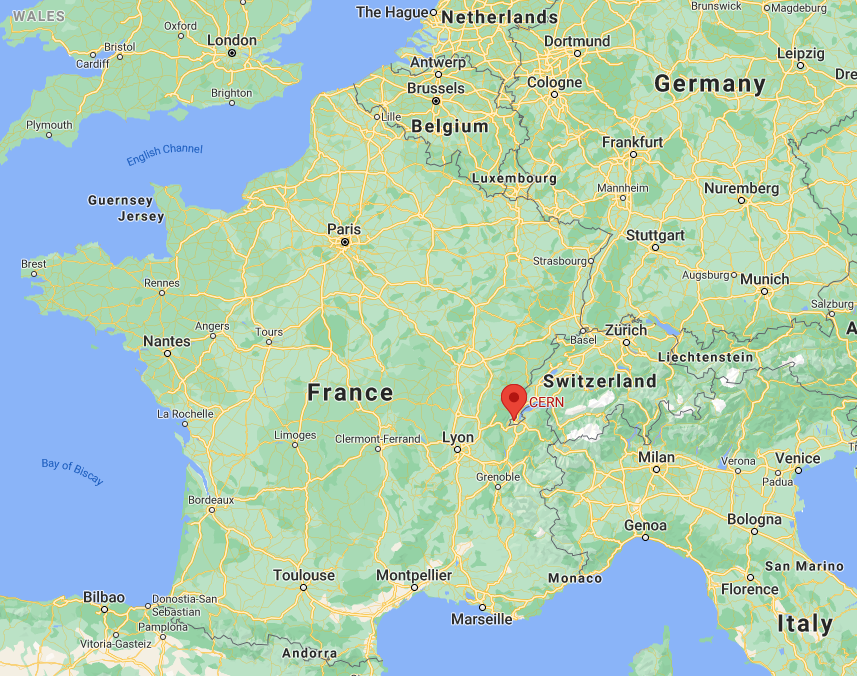
\includegraphics[width=.99\textwidth]{\PhDthesisdir/plots_and_images/CERN_and_LHC/maps-en.png}
\end{center}
\end{minipage}
\hfill
\begin{minipage}[c]{.5\textwidth}
\begin{center}
\begin{tikzpicture}
\node[anchor=south west,inner sep=0] at (0,0) {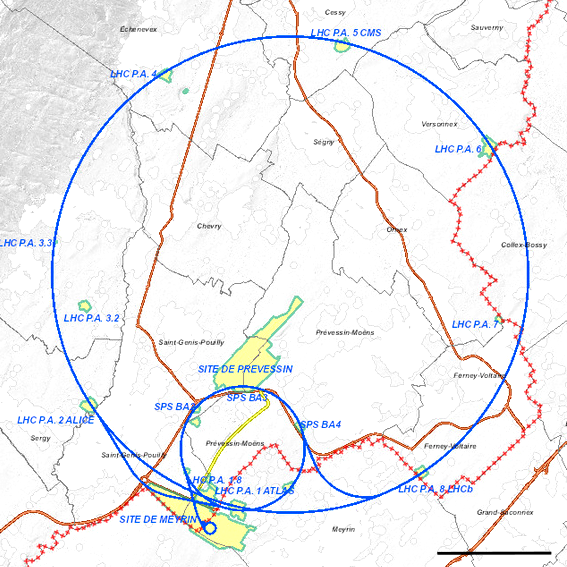
\includegraphics[scale=.35]{\PhDthesisdir/slides/LHC-CMS/LHC/CERN_LHC_map-scale_2km.png}};
\draw (6.125,.4) node {\SI{2}{\kilo\meter}};
\draw (2.95,.75) coordinate (LHCp1);
\draw (1.125,2) coordinate (LHCp2);
\draw (.65,4) coordinate (LHCp3);
\draw (1,3.2) coordinate (LHCp32);
\draw (2,6.1) coordinate (LHCp4);
\draw (4.25,6.45) coordinate (LHCp5);
\draw (6.05,5.15) coordinate (LHCp6);
\draw (6.15,3.125) coordinate (LHCp7);
\draw (5.15,1.15) coordinate (LHCp8);
\draw (LHCp1) coordinate (ATLAS);
\draw (LHCp2) coordinate (ALICE);
\draw (LHCp5) coordinate (CMS);
\draw (LHCp8) coordinate (LHCb);

%\foreach \coord in {1,2,3,4,5,6,7,8,32}{
%\fill[ltcolorred] (LHCp\coord) circle (3pt);
%}

%\draw [ultra thick, ltcolorred] (3.575,3.625) circle (2.95) ;
%\draw [ultra thick, ltcolorred] (3,1.475) circle (.75) ;
%\draw [ultra thick, ltcolorred] (2.6,.5) circle (.075) ;
%\fill [ltcolorred] (2.55,.55) circle (.05) ;
%\draw [ultra thick, ltcolorred] (2.5,.5) --+ (-60:.15) ;
\fill[ltcolorred] (CMS) circle (3pt);
\draw [ltcolorred4] (CMS) node [below] {\textbf{CMS}};
\fill[ltcolorred] (ATLAS) circle (3pt);
\draw [ltcolorred4] (ATLAS) node [above] {\textbf{ATLAS}};
\fill[ltcolorred] (ALICE) circle (3pt);
\draw [ltcolorred4] (ALICE) node [above right] {\textbf{ALICE}};
\fill[ltcolorred] (LHCb) circle (3pt);
\draw [ltcolorred4] (LHCb) node [below right] {\textbf{LHCb}};
\end{tikzpicture}
\end{center}
\end{minipage}
\end{frame}


\subsection{The CMS detector}
%\begin{frame}
\frametitle{The CMS detector}
\end{frame}
\begin{frame}\addtocounter{framenumber}{-1}
\frametitle{The CMS detector -- Silicon tracker (pixels)}
\begin{center}
detects charged particles going through

\vfill

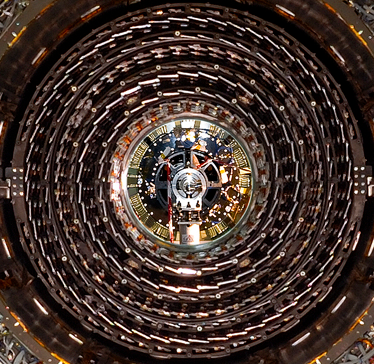
\includegraphics[width=\textwidth,height=0.75\textheight,keepaspectratio]{\PhDthesisdir/slides/LHC-CMS/CMS/CMS_zoomout_pictures/CMS_slice_photo_1-trk1.png}

\vfill

$\longleftarrow \SI{1}{\meter} \longrightarrow$
\end{center}
\end{frame}
\begin{frame}\addtocounter{framenumber}{-1}
\frametitle{The CMS detector -- Silicon tracker (strips)}
\begin{center}
detects charged particles going through

\vfill

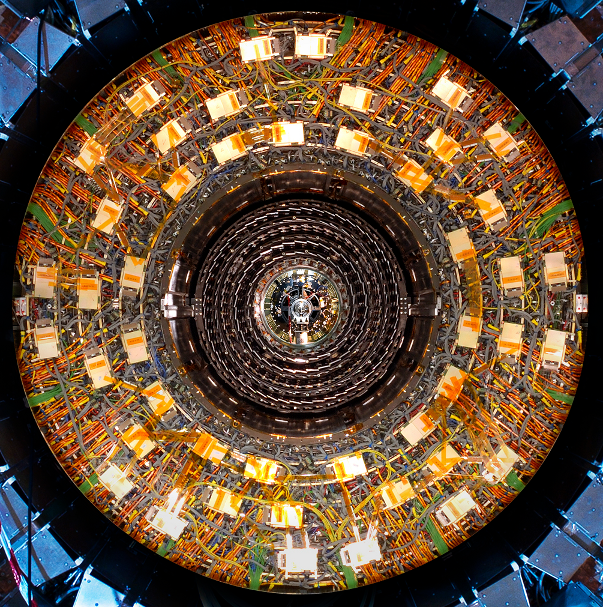
\includegraphics[width=\textwidth,height=0.75\textheight,keepaspectratio]{\PhDthesisdir/slides/LHC-CMS/CMS/CMS_zoomout_pictures/CMS_slice_photo_2-trk2.png}

\vfill

$\longleftarrow \SI{2}{\meter} \longrightarrow$
\end{center}
\end{frame}
\begin{frame}\addtocounter{framenumber}{-1}
\frametitle{The CMS detector -- Electromagnetic calorimeter (ECAL)}
\begin{center}
stops photons and electrons, measure their energies

\vfill

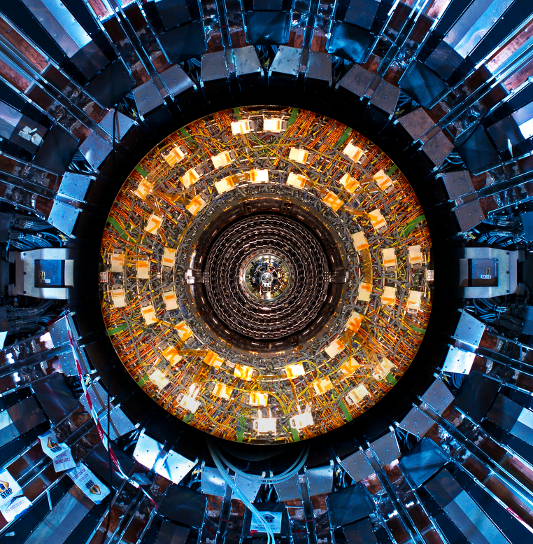
\includegraphics[width=\textwidth,height=0.75\textheight,keepaspectratio]{\PhDthesisdir/slides/LHC-CMS/CMS/CMS_zoomout_pictures/CMS_slice_photo_3-ECAL.png}

\vfill

$\longleftarrow \SI{3}{\meter} \longrightarrow$
\end{center}
\end{frame}
\begin{frame}\addtocounter{framenumber}{-1}
\frametitle{The CMS detector -- Hadron calorimeter (HCAL)}
\begin{center}
stops hadrons (protons, neutrons, ...), measure their energies

\vfill

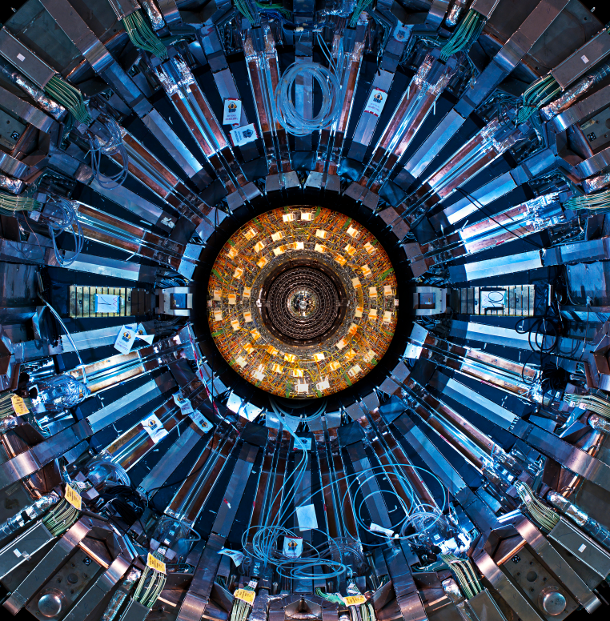
\includegraphics[width=\textwidth,height=0.75\textheight,keepaspectratio]{\PhDthesisdir/slides/LHC-CMS/CMS/CMS_zoomout_pictures/CMS_slice_photo_4-HCAL.png}

\vfill

$\longleftarrow \SI{5}{\meter} \longrightarrow$
\end{center}
\end{frame}
\begin{frame}\addtocounter{framenumber}{-1}
\frametitle{The CMS detector -- Superconducting solenoid}
\begin{center}
creates a \SI{4}{\tesla} magnetic field which bends charged particles trajectories

\vfill

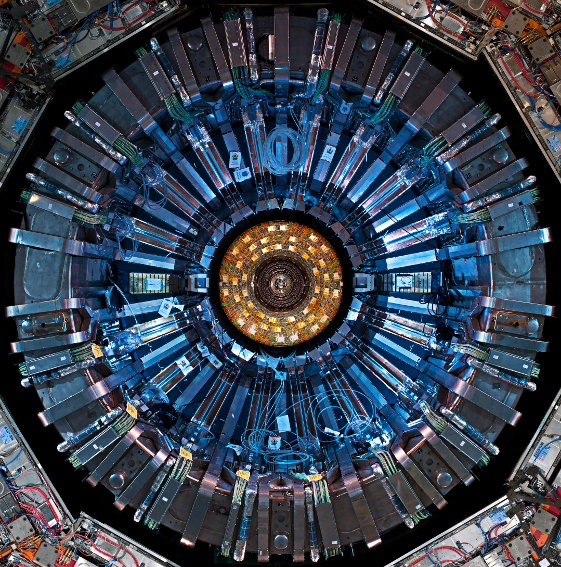
\includegraphics[width=\textwidth,height=0.75\textheight,keepaspectratio]{\PhDthesisdir/slides/LHC-CMS/CMS/CMS_zoomout_pictures/CMS_slice_photo_5-solenoid.png}

\vfill

$\longleftarrow \SI{7}{\meter} \longrightarrow$
\end{center}
\end{frame}
\begin{frame}\addtocounter{framenumber}{-1}
\frametitle{The CMS detector -- Muon system}
\begin{center}
detects muons going through

\vfill

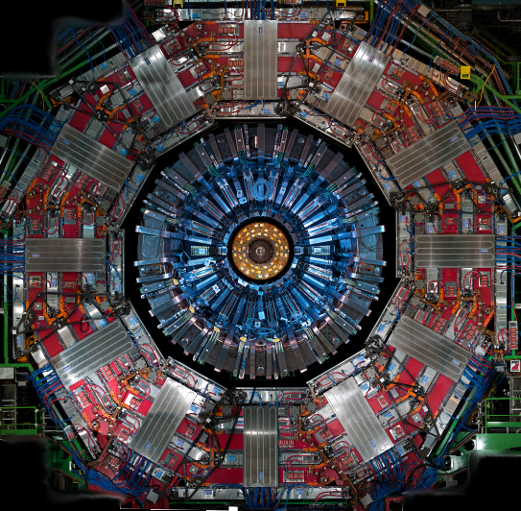
\includegraphics[width=\textwidth,height=0.75\textheight,keepaspectratio]{\PhDthesisdir/slides/LHC-CMS/CMS/CMS_zoomout_pictures/CMS_slice_photo_6-muons.png}

\vfill

$\longleftarrow \SI{15}{\meter} \longrightarrow$
\end{center}
\end{frame}
%\begin{frame}\addtocounter{framenumber}{-1}
\frametitle{The CMS detector}
\begin{center}
\vphantom{detects muons going through}

\vfill

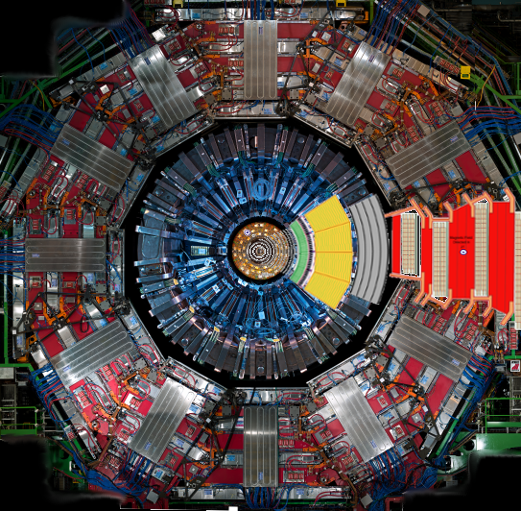
\includegraphics[width=\textwidth,height=0.75\textheight,keepaspectratio]{\PhDthesisdir/plots_and_images/CMS_slices/own/slice_on_photo.tex}

\vfill

$\longleftarrow \SI{15}{\meter} \longrightarrow$
\end{center}
\end{frame}
\begin{frame}
\begin{minipage}[t]{.6\textwidth}
\begin{figure}
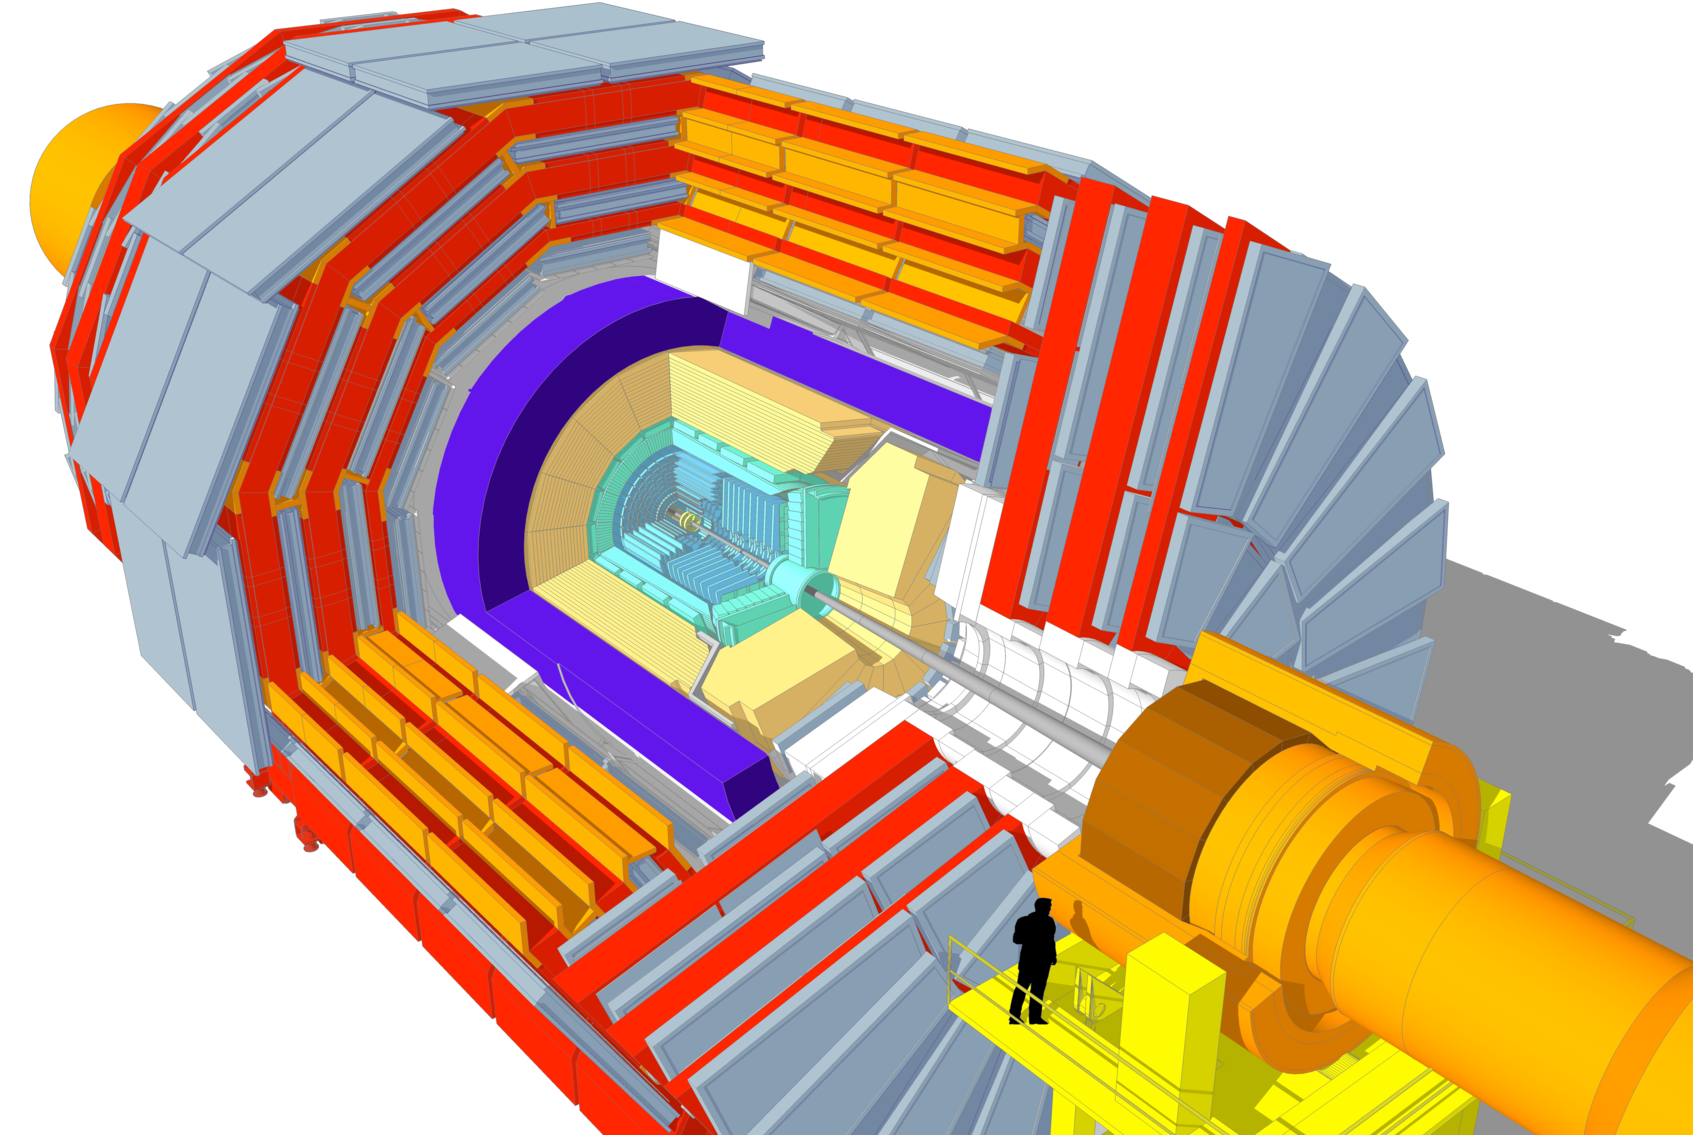
\includegraphics[width=\textwidth,height=\graphh,keepaspectratio]{\PhDthesisdir/plots_and_images/CMS_slices/from_CMS_document_11982-v2/small_cms_full.png}
\end{figure}
\end{minipage}
\hfill\begin{minipage}[t]{.35\textwidth}
\begin{block}{CMS detector}
\begin{itemize}
\item Mass: $\sim\SI{14000}{t}$, $\num{12500}$ only for red part
\item Diameter: \SI{15}{\meter}
\item Length: \SI{28.7}{\meter}
\end{itemize}
\end{block}

\begin{block}{}
$\Rightarrow$ How to \emph{see} the particles?
\end{block}
\end{minipage}
\end{frame}

\begin{frame}
\addtocounter{framenumber}{-1}
%\transdissolve
\begin{minipage}[t]{.6\textwidth}
\begin{figure}
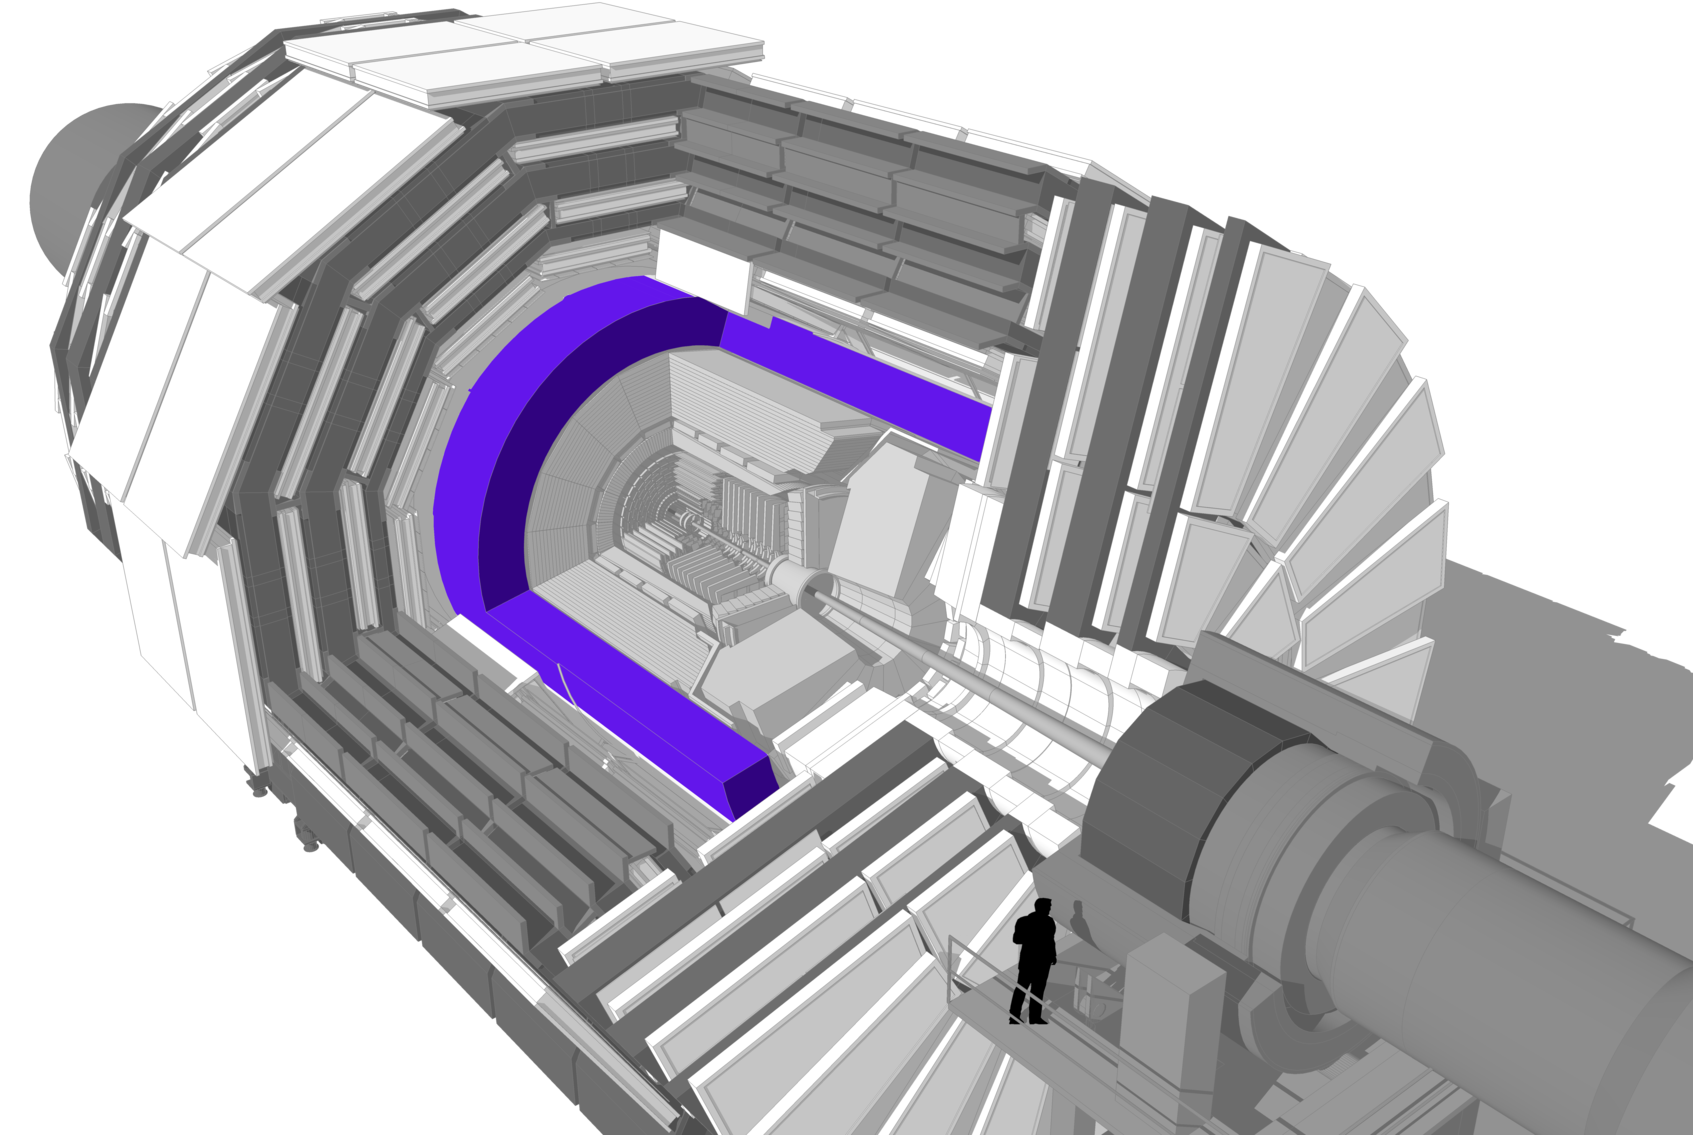
\includegraphics[width=\textwidth,height=\graphh,keepaspectratio]{\PhDthesisdir/plots_and_images/CMS_slices/from_CMS_document_11982-v2/small_cms_solenoid.png}
\end{figure}
\end{minipage}
\hfill\begin{minipage}[t]{.35\textwidth}
\begin{block}{Solenoid}
\begin{itemize}
\item Niobium titanium coil
\item Superconducting
\item $\sim\SI{18000}{\ampere}$
\item \SI{4}{\tesla} in the inner volume
\end{itemize}
\end{block}

\begin{block}{}
$\Rightarrow$ Bends charged particles trajectories in the transverse plane
\end{block}
\end{minipage}
\end{frame}

\begin{frame}
\addtocounter{framenumber}{-1}
%\transdissolve
\begin{minipage}[t]{.6\textwidth}
\begin{figure}
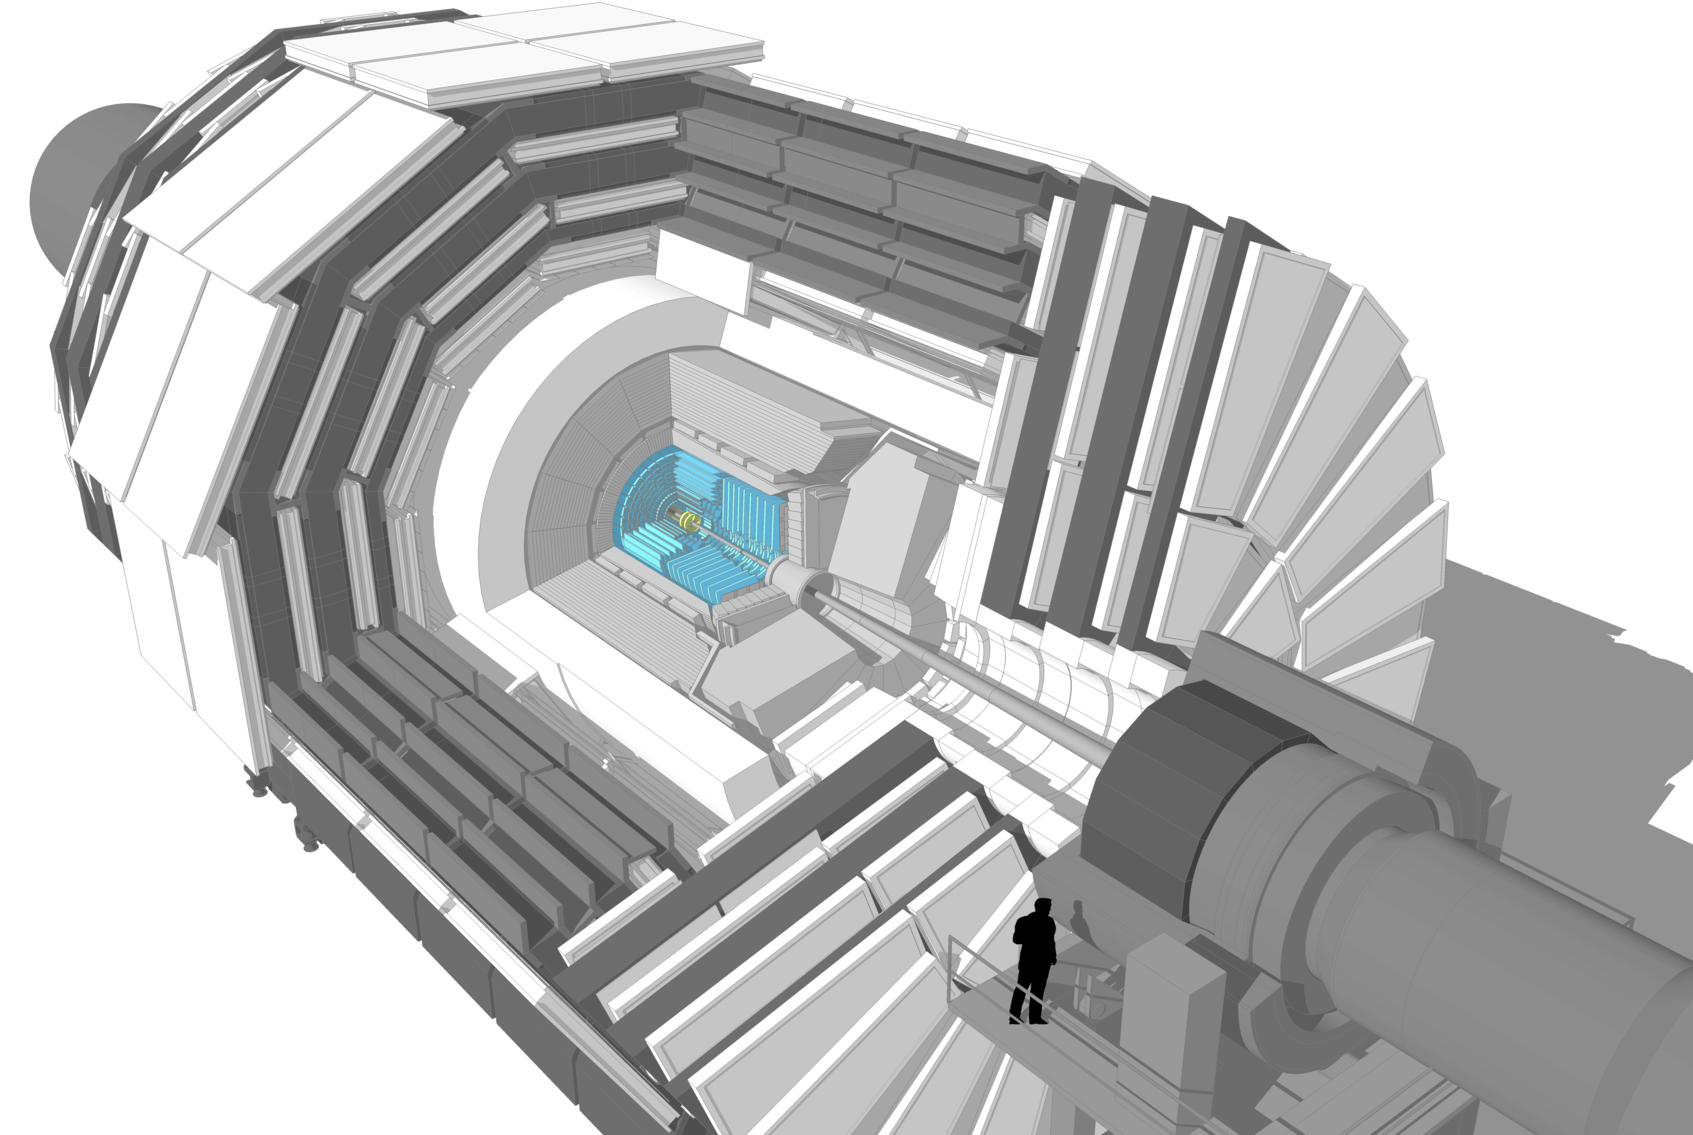
\includegraphics[width=\textwidth,height=\graphh,keepaspectratio]{\PhDthesisdir/plots_and_images/CMS_slices/from_CMS_document_11982-v2/small_cms_tracker.png}
\end{figure}
\end{minipage}
\hfill\begin{minipage}[t]{.35\textwidth}
\begin{block}{Tracker}
\begin{itemize}
\item Inner: pixels ($\num{100}\times\SI{150}{\micro\meter^2}$, $\sim\SI{1.9}{\meter^2}$, $\sim\SI{124}{M}$ channels
\item Outer: microstrips ($\num{80}-\SI{180}{\micro\meter}$) $\sim\SI{200}{\meter^2}$ $\sim\SI{9.6}{M}$ channels
\end{itemize}
\end{block}

\begin{block}{}
$\Rightarrow$ Charged particles leave hits when going through
\end{block}
\end{minipage}
\end{frame}

\begin{frame}
\addtocounter{framenumber}{-1}
%\transdissolve
\begin{minipage}[t]{.6\textwidth}
\begin{figure}
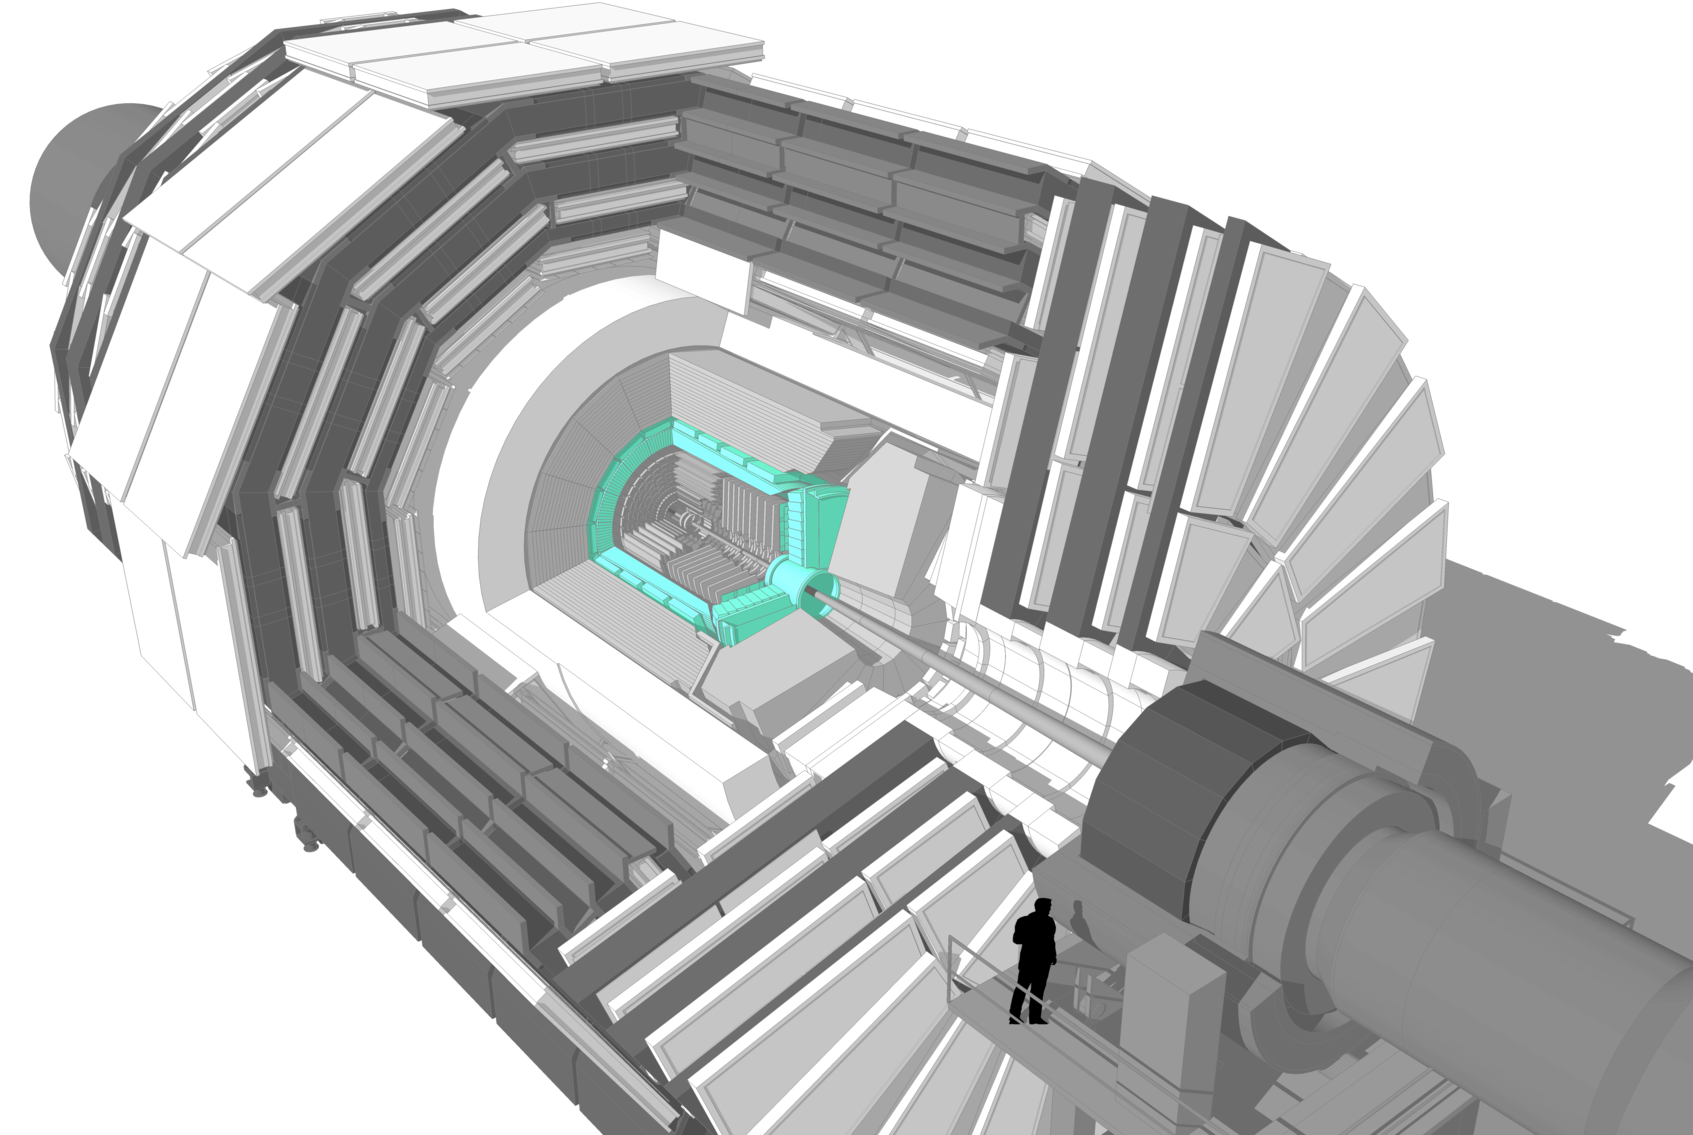
\includegraphics[width=\textwidth,height=\graphh,keepaspectratio]{\PhDthesisdir/plots_and_images/CMS_slices/from_CMS_document_11982-v2/small_cms_ecal.png}
\end{figure}
\end{minipage}
\hfill\begin{minipage}[t]{.35\textwidth}
\begin{block}{Electromagnetic CALorimeter}
\begin{itemize}
\item $\sim\num{76000}$ scintillating \ce{PbWO4} crystals
\end{itemize}
\end{block}

\begin{block}{}
$\Rightarrow$ electrons and photons are stopped, energy deposits
\end{block}
\end{minipage}
\end{frame}

\begin{frame}
\addtocounter{framenumber}{-1}
%\transdissolve
\begin{minipage}[t]{.6\textwidth}
\begin{figure}
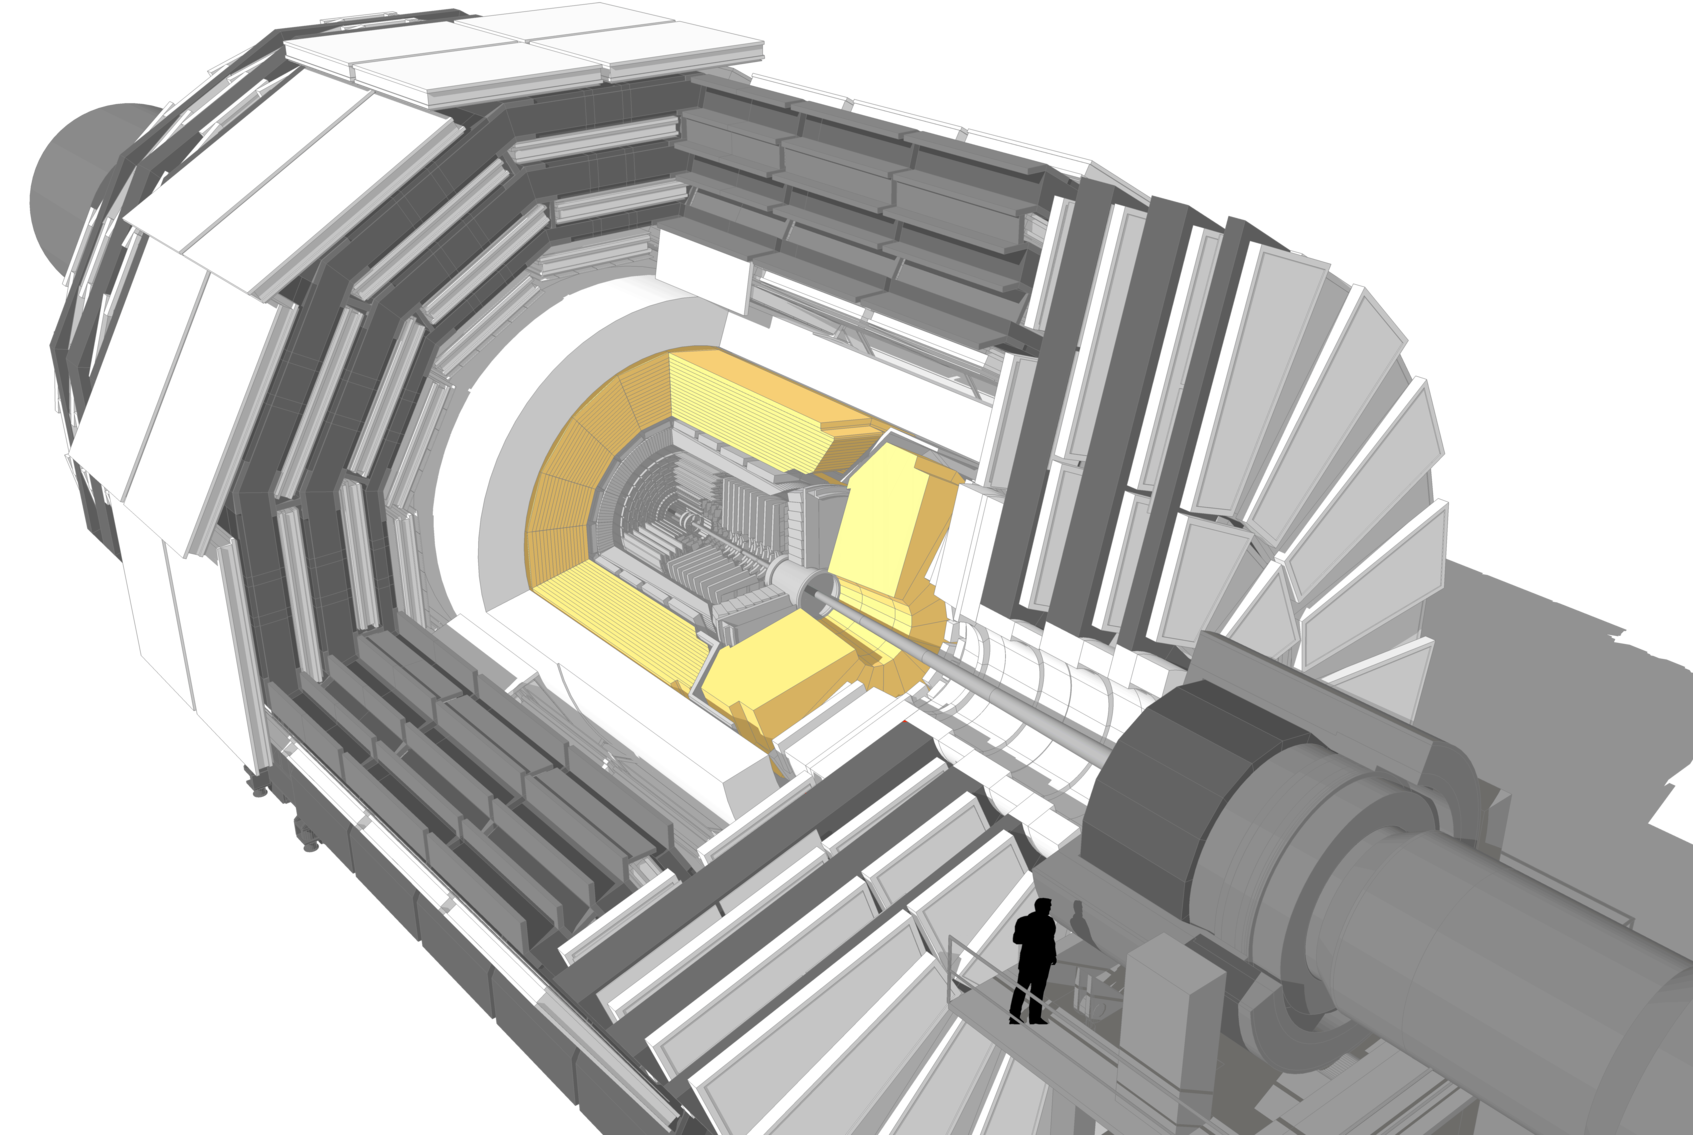
\includegraphics[width=\textwidth,height=\graphh,keepaspectratio]{\PhDthesisdir/plots_and_images/CMS_slices/from_CMS_document_11982-v2/small_cms_hcal.png}
\end{figure}
\end{minipage}
\hfill\begin{minipage}[t]{.35\textwidth}
\begin{block}{Hadronic CALorimeter (yellow)}
\begin{itemize}
\item brass + plastic scintillator, $\sim\num{7000}$ channels
\end{itemize}
\end{block}

\begin{block}{Forward CALorimeter (orange)}
\begin{itemize}
\item steel + quartz fibres, $\sim\num{2000}$ channels
\end{itemize}
\end{block}

\begin{block}{}
$\Rightarrow$ hadrons are stopped, energy deposits
\end{block}
\end{minipage}
\end{frame}

\begin{frame}
\addtocounter{framenumber}{-1}
%\transdissolve
\begin{minipage}[t]{.6\textwidth}
\begin{figure}
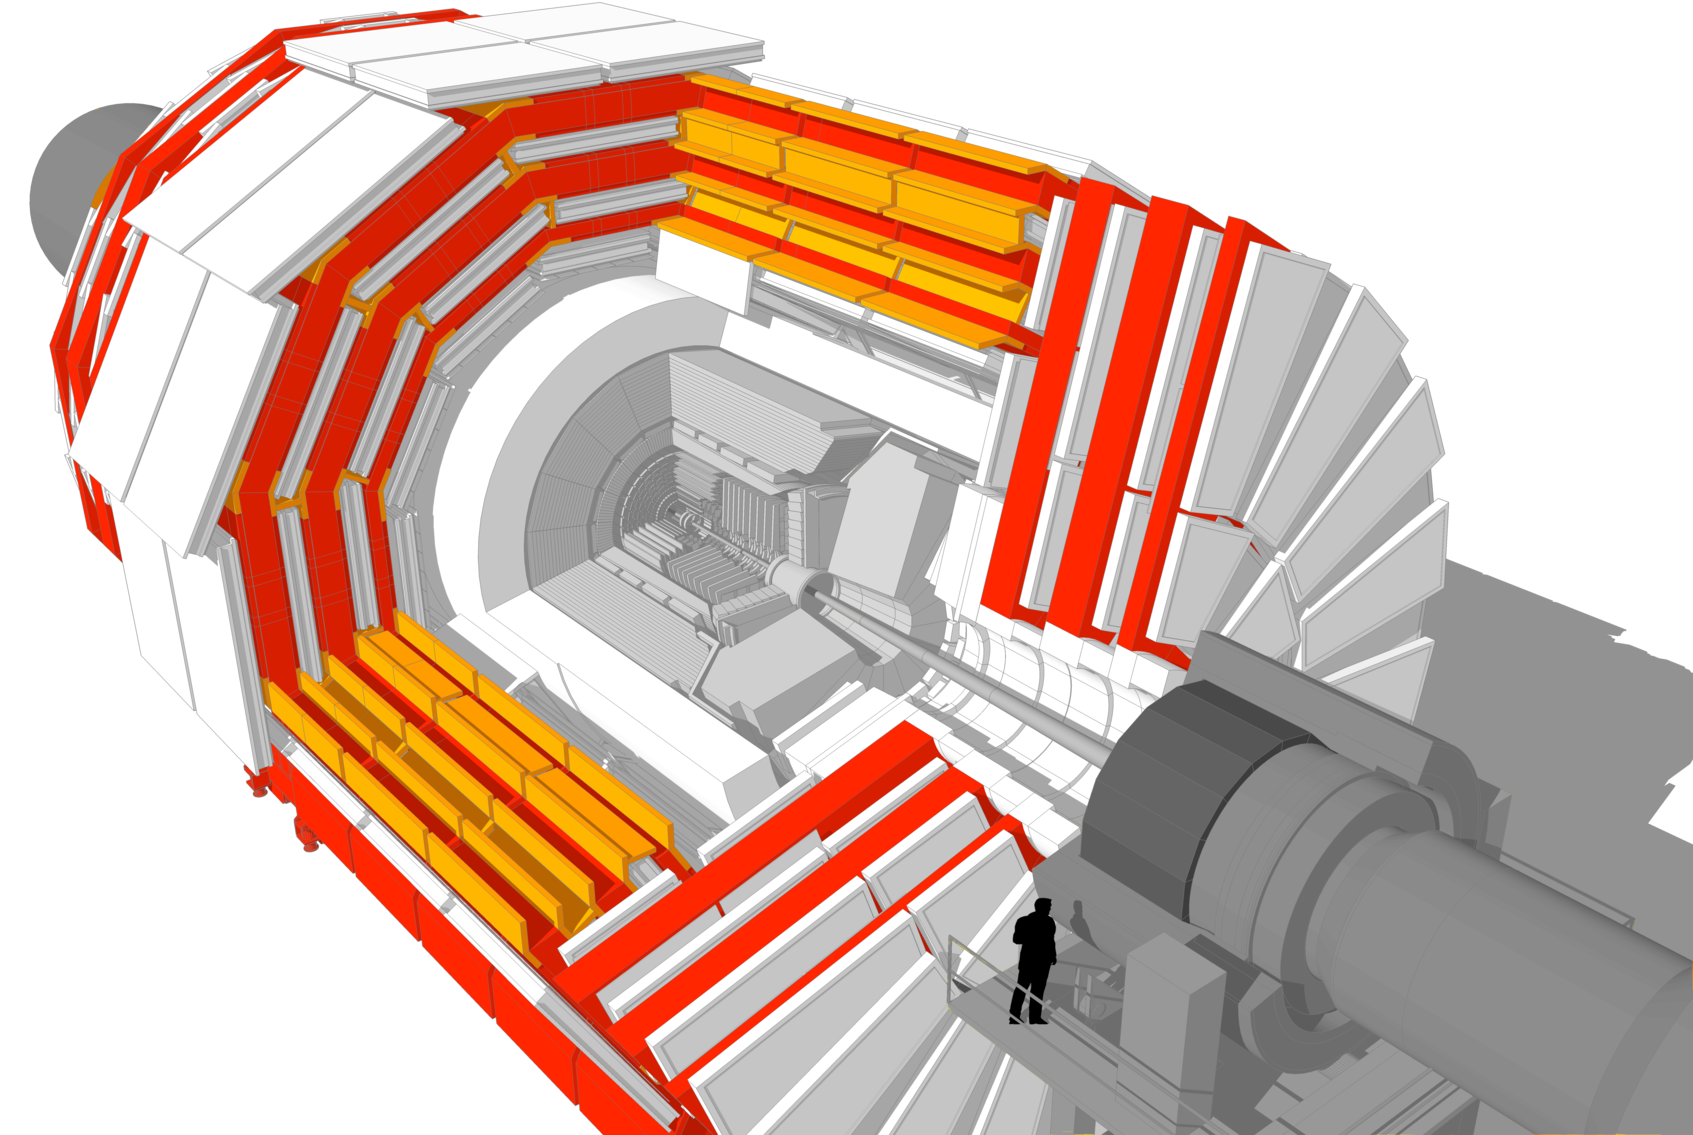
\includegraphics[width=\textwidth,height=\graphh,keepaspectratio]{\PhDthesisdir/plots_and_images/CMS_slices/from_CMS_document_11982-v2/small_cms_muons.png}
\end{figure}
\end{minipage}
\hfill\begin{minipage}[t]{.35\textwidth}
\begin{block}{Steel return yoke (red)}
\begin{itemize}
\item allows for \SI{2}{\tesla} magnetic field around the solenoid
\end{itemize}
\end{block}

\begin{block}{Muon chambers (blue-gray)}
\begin{itemize}
\item Barrel: \num{250} drift tubes, \num{480} resistive plate chambers
\item Endcaps: \num{540} cathode strip, \num{576} resistive plate chambers
\end{itemize}
\end{block}

\begin{block}{}
$\Rightarrow$ charged particles leave hits when going through (only muons do)
\end{block}
\vspace{-2\baselineskip}
\end{minipage}
\end{frame}

\begin{frame}
\addtocounter{framenumber}{-1}
%\transdissolve
\begin{minipage}[t]{.6\textwidth}
\begin{figure}
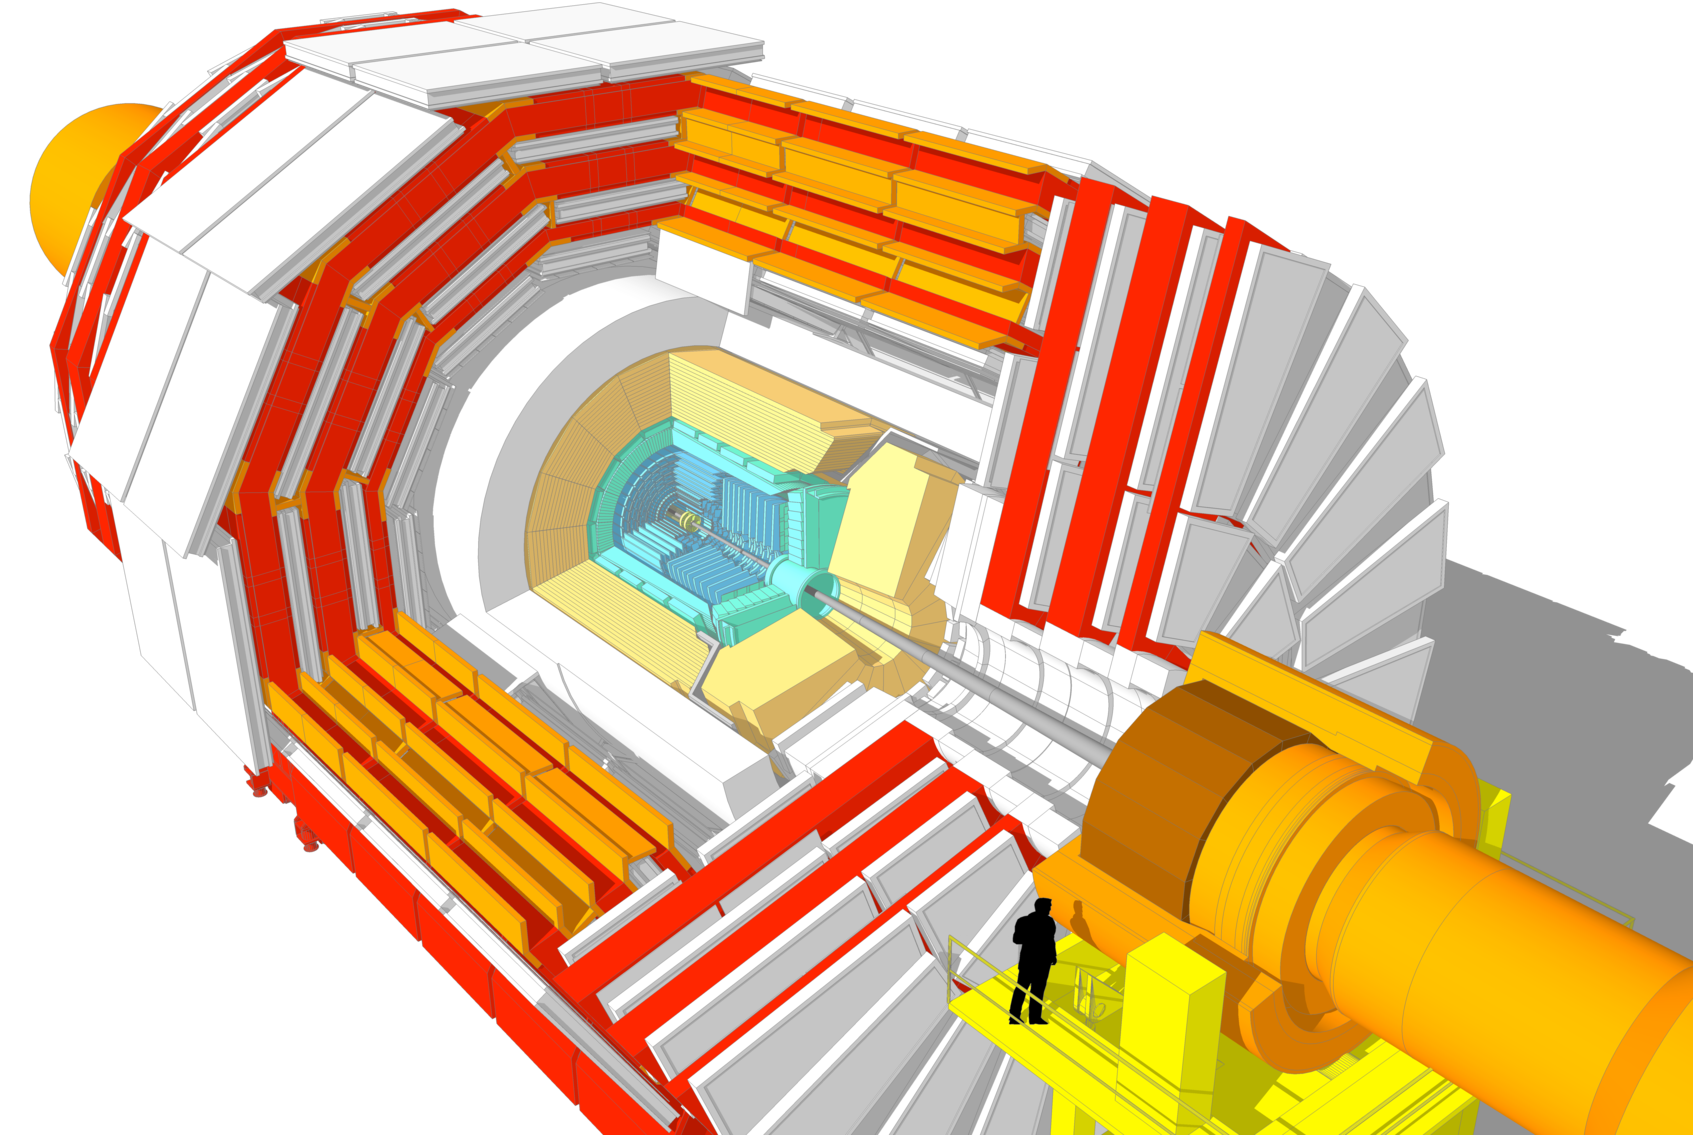
\includegraphics[width=\textwidth,height=\graphh,keepaspectratio]{\PhDthesisdir/plots_and_images/CMS_slices/from_CMS_document_11982-v2/small_cms_full_no_violet_solen.png}
\end{figure}
\end{minipage}
\hfill\begin{minipage}[t]{.35\textwidth}
\begin{block}{Sensitive parts of CMS}
Combine sub-detectors signals to determine which particles were there!
\end{block}
\end{minipage}
\end{frame}
\begin{frame}
\transdissolve
\transduration{0}
\end{frame}

\begin{frame}
\transwipe
\transduration{0}
\begin{center}
\includegraphics[width=\textwidth,height=\graphh,keepaspectratio]{\PhDthesisdir/plots_and_images/CMS_slices/own/cms_slice_CMS_parts/1-only_cms_size.tex}
\end{center}
\end{frame}

\begin{frame}
\addtocounter{framenumber}{-1}
\transdissolve[duration=2]
\transduration{0}
\begin{center}
\includegraphics[width=\textwidth,height=\graphh,keepaspectratio]{\PhDthesisdir/plots_and_images/CMS_slices/own/cms_slice_CMS_parts/2-add_trk.tex}
\end{center}
\end{frame}

\begin{frame}
\addtocounter{framenumber}{-1}
\transdissolve[duration=2]
\transduration{0}
\begin{center}
\includegraphics[width=\textwidth,height=\graphh,keepaspectratio]{\PhDthesisdir/plots_and_images/CMS_slices/own/cms_slice_CMS_parts/3-add_ECAL.tex}
\end{center}
\end{frame}

\begin{frame}
\addtocounter{framenumber}{-1}
\transdissolve[duration=2]
\transduration{0}
\begin{center}
\includegraphics[width=\textwidth,height=\graphh,keepaspectratio]{\PhDthesisdir/plots_and_images/CMS_slices/own/cms_slice_CMS_parts/4-add_HCAL.tex}
\end{center}
\end{frame}

\begin{frame}
\addtocounter{framenumber}{-1}
\transdissolve[duration=2]
\transduration{0}
\begin{center}
\includegraphics[width=\textwidth,height=\graphh,keepaspectratio]{\PhDthesisdir/plots_and_images/CMS_slices/own/cms_slice_CMS_parts/5-add_solen.tex}
\end{center}
\end{frame}

%\begin{frame}
%\addtocounter{framenumber}{-1}
%\transdissolve
%\transduration{0}
%\begin{center}
%\includegraphics[width=\textwidth,height=\graphh,keepaspectratio]{\PhDthesisdir/plots_and_images/CMS_slices/own/cms_slice_CMS_parts/6-1-add_iron_RY.tex}
%\end{center}
%\end{frame}
%
%\begin{frame}
%\addtocounter{framenumber}{-1}
%\transdissolve
%\transduration{0}
%\begin{center}
%\includegraphics[width=\textwidth,height=\graphh,keepaspectratio]{\PhDthesisdir/plots_and_images/CMS_slices/own/cms_slice_CMS_parts/6-2-add_muon1.tex}
%\end{center}
%\end{frame}
%
%\begin{frame}
%\addtocounter{framenumber}{-1}
%\transdissolve
%\transduration{0}
%\begin{center}
%\includegraphics[width=\textwidth,height=\graphh,keepaspectratio]{\PhDthesisdir/plots_and_images/CMS_slices/own/cms_slice_CMS_parts/6-3-add_muon2.tex}
%\end{center}
%\end{frame}
%
%\begin{frame}
%\addtocounter{framenumber}{-1}
%\transdissolve
%\transduration{0}
%\begin{center}
%\includegraphics[width=\textwidth,height=\graphh,keepaspectratio]{\PhDthesisdir/plots_and_images/CMS_slices/own/cms_slice_CMS_parts/6-4-add_muon3.tex}
%\end{center}
%\end{frame}

\begin{frame}
\addtocounter{framenumber}{-1}
\transdissolve[duration=2]
\transduration{0}
\begin{center}
\includegraphics[width=\textwidth,height=\graphh,keepaspectratio]{\PhDthesisdir/plots_and_images/CMS_slices/own/cms_slice_CMS_parts/6-5-add_muon4.tex}
\end{center}
\end{frame}

%\begin{frame}
%\addtocounter{framenumber}{-1}
%\transdissolve[duration=2]
%\transduration{0}
%\begin{center}
%\includegraphics[width=\textwidth,height=\graphh,keepaspectratio]{\PhDthesisdir/plots_and_images/CMS_slices/own/cms_slice_CMS_parts/7-add_B_field.tex}
%\end{center}
%\end{frame}

\begin{frame}
\addtocounter{framenumber}{-1}
\transdissolve[duration=2]
\transduration{0}
\begin{center}
\includegraphics[width=\textwidth,height=\graphh,keepaspectratio]{\PhDthesisdir/plots_and_images/CMS_slices/own/cms_slice_particles_appear/0-nothing.tex}
\end{center}
\end{frame}

%\begin{frame}
%\addtocounter{framenumber}{-1}
%\transwipe
%\transduration{0}
%\begin{center}
%\includegraphics[width=\textwidth,height=\graphh,keepaspectratio]{\PhDthesisdir/plots_and_images/CMS_slices/own/cms_slice_particles_appear/1-up_to_CH.tex}
%\end{center}
%\end{frame}
%
%\begin{frame}
%\addtocounter{framenumber}{-1}
%\transwipe
%\transduration{0}
%\begin{center}
%\includegraphics[width=\textwidth,height=\graphh,keepaspectratio]{\PhDthesisdir/plots_and_images/CMS_slices/own/cms_slice_particles_appear/2-up_to_NH.tex}
%\end{center}
%\end{frame}
%
%\begin{frame}
%\addtocounter{framenumber}{-1}
%\transwipe
%\transduration{0}
%\begin{center}
%\includegraphics[width=\textwidth,height=\graphh,keepaspectratio]{\PhDthesisdir/plots_and_images/CMS_slices/own/cms_slice_particles_appear/3-up_to_photon.tex}
%\end{center}
%\end{frame}
%
%\begin{frame}
%\addtocounter{framenumber}{-1}
%\transwipe
%\transduration{0}
%\begin{center}
%\includegraphics[width=\textwidth,height=\graphh,keepaspectratio]{\PhDthesisdir/plots_and_images/CMS_slices/own/cms_slice_particles_appear/4-up_to_ele.tex}
%\end{center}
%\end{frame}

\begin{frame}
\addtocounter{framenumber}{-1}
\transwipe
\begin{center}
\includegraphics[width=\textwidth,height=\graphh,keepaspectratio]{\PhDthesisdir/plots_and_images/CMS_slices/own/all_ptcs.tex}
\end{center}
\end{frame}
%\begin{frame}
\frametitle{Neutrinos and missing transverse energy (MET)}

\begin{center}
\begin{tikzpicture}
\def\trackerrin{.100}
\def\trackerrout{1.185}
\def\trackercolor{ltcolorgray1}

\def\ECALrin{1.290}
\def\ECALrout{1.811}
\def\ECALcolor{ltcolorgreen1}

\def\HCALrin{1.812}
\def\HCALrout{2.854}
\def\HCALcolor{ltcoloryellow3}

\def\Solenrin{2.950}
\def\Solenrout{3.800}
\def\Solencolor{ltcolorgray2}

\def\ironryrina{3.850}
\def\ironryrouta{4.000}
\def\muonrina{4.020}
\def\muonrouta{4.400}
\def\ironryrinb{4.420}
\def\ironryroutb{4.880}
\def\muonrinb{4.905}
\def\muonroutb{5.285}
\def\ironryrinc{5.300}
\def\ironryroutc{5.960}
\def\muonrinc{5.975}
\def\muonroutc{6.355}
\def\ironryrind{6.375}
\def\ironryroutd{6.980}
\def\muonrind{7.000}
\def\muonroutd{7.380}
\def\muoncolor{ltcoloryellow1}
\def\ironrycolor{ltcolorred2}

\def\printele#1{
\draw [thick, ltcolorred] (0,0) arc (#1-90:#1-90+27:3) coordinate (eledeposit);
\draw [ltcolorred] (#1-5:1.25) node {\ele};
}
\def\printmu#1{
\draw [thick, ltcolorblue] (0,0) arc (#1-90:#1-90+33:6) arc (#1-90+33:#1-90:-12) node{\mu};
\draw [ltcolorblue] (#1-7:1.5) node {\mu};
}

\def\printantiele#1{
\draw [thick, ltcolorred] (0,0) arc (#1-90:#1-90-27:-3) coordinate (eledeposit);
\draw [ltcolorred] (#1-7:1.5) node {\ele};
%\draw [ltcolorred4, ultra thick] (eledeposit)--+(#1+25:\ECALrout);
}
\def\printantimu#1{
\draw [thick, ltcolorblue] (0,0) arc (#1-90:#1-90-33:-6) arc (#1-90-33:#1-90:12);
\draw [ltcolorblue] (#1-7:1.5) node {\mu};
}

\def\printtauh#1{
\draw [thick, ltcolorgreen4] (0,0) arc (#1-90:#1-90+11:10) ;
\draw [thick, ltcolorgreen4] (0,0) arc (#1-90:#1-90+6:20) ;
\draw [thick, ltcolorgreen4] (0,0) arc (#1-90:#1-90-11:-10) ;
\draw [ltcolorgreen4] (#1-12:1.5) node {\tauh};
}
\def\printantitauh#1{
\draw [thick, ltcolorgreen4] (0,0) arc (#1-90:#1-90-11:-10) ;
\draw [thick, ltcolorgreen4] (0,0) arc (#1-90:#1-90-6:-20) ;
\draw [thick, ltcolorgreen4] (0,0) arc (#1-90:#1-90+11:10) ;
\draw [ltcolorgreen4] (#1-12:1.5) node {\tauh};
}

\def\printjetnolabel#1{
\draw [thick, ltcolororange] (0,0) arc (#1-90+10:#1-90+22+10:5) ;
\draw [thick, ltcolororange] (0,0) arc (#1-90+5:#1-90+12+5:10) ;
\draw [thick, ltcolororange] (0,0) arc (#1-90:#1-90-22:-5) ;
\draw [thick, ltcolororange] (0,0) arc (#1-90:#1-90+6:20) ;
\draw [thick, ltcolororange] (0,0) arc (#1-90+5:#1-90+8+5:10) ;
\draw [thick, ltcolororange] (0,0) arc (#1-90:#1-90-11:-10) ;
\draw [thick, ltcolororange] (0,0) arc (#1-90:#1-90+11:10) ;
}

\def\printjet#1{
\printjetnolabel{#1}
\draw [ltcolororange] (#1-25:.5) node {jet};
}

\def\printjetfake#1{
\printjet{#1}
\draw [thick, ltcolorgreen4] (0,0) arc (#1-90:#1-90+11:10) ;
\draw [thick, ltcolorgreen4] (0,0) arc (#1-90:#1-90+6:20) ;
\draw [thick, ltcolorgreen4] (0,0) arc (#1-90:#1-90-11:-10) ;
\draw [ltcolorgreen4] (#1-17:1.5) node {f.\tauh};
}

\def\printdeposit#1#2#3#4{
\fill [#1] (#2-2:#3) arc (#2-2:#2+2:#3) -- (#2+2:#4) arc (#2+2:#2-2:#4) ;
}

\def\printECALdeposit#1#2{\printdeposit{#1}{#2}{\ECALrin}{\ECALrout}}
\def\printHCALdeposit#1#2{\printdeposit{#1}{#2}{\HCALrin}{\HCALrout}}

\def\printtauhdeposit#1{
\printHCALdeposit{ltcoloryellow4}{#1+3}
\printHCALdeposit{ltcoloryellow4}{#1+5}
\printHCALdeposit{ltcoloryellow4}{#1-5}
}

\def\printjetdeposit#1{
\printHCALdeposit{ltcoloryellow4}{#1+3}
\printHCALdeposit{ltcoloryellow4}{#1+5}
\printHCALdeposit{ltcoloryellow4}{#1-5}
\printHCALdeposit{ltcoloryellow4}{#1+21}
\printHCALdeposit{ltcoloryellow4}{#1+11}
\printHCALdeposit{ltcoloryellow4}{#1-11}
}

\def\printMuChSigA#1#2{
\fill [red] (#1-7.5+20*#2:\muonrina) arc (#1-7.5+20*#2:#1+7.5+20*#2:\muonrina) -- (#1+7.5+20*#2:\muonrouta) arc (#1+7.5+20*#2:#1-7.5+20*#2:\muonrouta) ;
}
\def\printMuChSigB#1#2{
\fill [red] (#1-7.5+20*#2:\muonrinb) arc (#1-7.5+20*#2:#1+7.5+20*#2:\muonrinb) -- (#1+7.5+20*#2:\muonroutb) arc (#1+7.5+20*#2:#1-7.5+20*#2:\muonroutb) ;
}
\def\printMuChSigC#1#2{
\fill [red] (#1-7.5+20*#2:\muonrinc) arc (#1-7.5+20*#2:#1+7.5+20*#2:\muonrinc) -- (#1+7.5+20*#2:\muonroutc) arc (#1+7.5+20*#2:#1-7.5+20*#2:\muonroutc) ;
}
\def\printMuChSigD#1#2{
\fill [red] (#1-7.5+20*#2:\muonrind) arc (#1-7.5+20*#2:#1+7.5+20*#2:\muonrind) -- (#1+7.5+20*#2:\muonroutd) arc (#1+7.5+20*#2:#1-7.5+20*#2:\muonroutd) ;
}

\clip (-\graphw/2,-\graphh/2) rectangle (\graphw/2,\graphh/2);

\printjetnolabel{60}
\printjetnolabel{40}

%\draw [thick, -latex, ltcolorred] (0,0)--+(-130:\HCALrout) node [below] {\vMET};

\fill (0,0) circle (2pt);
\end{tikzpicture}
\end{center}

\end{frame}

\begin{frame}\addtocounter{framenumber}{-1}
\frametitle{Neutrinos and missing transverse energy (MET)}

\begin{center}
\begin{tikzpicture}
\def\trackerrin{.100}
\def\trackerrout{1.185}
\def\trackercolor{ltcolorgray1}

\def\ECALrin{1.290}
\def\ECALrout{1.811}
\def\ECALcolor{ltcolorgreen1}

\def\HCALrin{1.812}
\def\HCALrout{2.854}
\def\HCALcolor{ltcoloryellow3}

\def\Solenrin{2.950}
\def\Solenrout{3.800}
\def\Solencolor{ltcolorgray2}

\def\ironryrina{3.850}
\def\ironryrouta{4.000}
\def\muonrina{4.020}
\def\muonrouta{4.400}
\def\ironryrinb{4.420}
\def\ironryroutb{4.880}
\def\muonrinb{4.905}
\def\muonroutb{5.285}
\def\ironryrinc{5.300}
\def\ironryroutc{5.960}
\def\muonrinc{5.975}
\def\muonroutc{6.355}
\def\ironryrind{6.375}
\def\ironryroutd{6.980}
\def\muonrind{7.000}
\def\muonroutd{7.380}
\def\muoncolor{ltcoloryellow1}
\def\ironrycolor{ltcolorred2}

\def\printele#1{
\draw [thick, ltcolorred] (0,0) arc (#1-90:#1-90+27:3) coordinate (eledeposit);
\draw [ltcolorred] (#1-5:1.25) node {\ele};
}
\def\printmu#1{
\draw [thick, ltcolorblue] (0,0) arc (#1-90:#1-90+33:6) arc (#1-90+33:#1-90:-12) node{\mu};
\draw [ltcolorblue] (#1-7:1.5) node {\mu};
}

\def\printantiele#1{
\draw [thick, ltcolorred] (0,0) arc (#1-90:#1-90-27:-3) coordinate (eledeposit);
\draw [ltcolorred] (#1-7:1.5) node {\ele};
%\draw [ltcolorred4, ultra thick] (eledeposit)--+(#1+25:\ECALrout);
}
\def\printantimu#1{
\draw [thick, ltcolorblue] (0,0) arc (#1-90:#1-90-33:-6) arc (#1-90-33:#1-90:12);
\draw [ltcolorblue] (#1-7:1.5) node {\mu};
}

\def\printtauh#1{
\draw [thick, ltcolorgreen4] (0,0) arc (#1-90:#1-90+11:10) ;
\draw [thick, ltcolorgreen4] (0,0) arc (#1-90:#1-90+6:20) ;
\draw [thick, ltcolorgreen4] (0,0) arc (#1-90:#1-90-11:-10) ;
\draw [ltcolorgreen4] (#1-12:1.5) node {\tauh};
}
\def\printantitauh#1{
\draw [thick, ltcolorgreen4] (0,0) arc (#1-90:#1-90-11:-10) ;
\draw [thick, ltcolorgreen4] (0,0) arc (#1-90:#1-90-6:-20) ;
\draw [thick, ltcolorgreen4] (0,0) arc (#1-90:#1-90+11:10) ;
\draw [ltcolorgreen4] (#1-12:1.5) node {\tauh};
}

\def\printjetnolabel#1{
\draw [thick, ltcolororange] (0,0) arc (#1-90+10:#1-90+22+10:5) ;
\draw [thick, ltcolororange] (0,0) arc (#1-90+5:#1-90+12+5:10) ;
\draw [thick, ltcolororange] (0,0) arc (#1-90:#1-90-22:-5) ;
\draw [thick, ltcolororange] (0,0) arc (#1-90:#1-90+6:20) ;
\draw [thick, ltcolororange] (0,0) arc (#1-90+5:#1-90+8+5:10) ;
\draw [thick, ltcolororange] (0,0) arc (#1-90:#1-90-11:-10) ;
\draw [thick, ltcolororange] (0,0) arc (#1-90:#1-90+11:10) ;
}

\def\printjet#1{
\printjetnolabel{#1}
\draw [ltcolororange] (#1-25:.5) node {jet};
}

\def\printjetfake#1{
\printjet{#1}
\draw [thick, ltcolorgreen4] (0,0) arc (#1-90:#1-90+11:10) ;
\draw [thick, ltcolorgreen4] (0,0) arc (#1-90:#1-90+6:20) ;
\draw [thick, ltcolorgreen4] (0,0) arc (#1-90:#1-90-11:-10) ;
\draw [ltcolorgreen4] (#1-17:1.5) node {f.\tauh};
}

\def\printdeposit#1#2#3#4{
\fill [#1] (#2-2:#3) arc (#2-2:#2+2:#3) -- (#2+2:#4) arc (#2+2:#2-2:#4) ;
}

\def\printECALdeposit#1#2{\printdeposit{#1}{#2}{\ECALrin}{\ECALrout}}
\def\printHCALdeposit#1#2{\printdeposit{#1}{#2}{\HCALrin}{\HCALrout}}

\def\printtauhdeposit#1{
\printHCALdeposit{ltcoloryellow4}{#1+3}
\printHCALdeposit{ltcoloryellow4}{#1+5}
\printHCALdeposit{ltcoloryellow4}{#1-5}
}

\def\printjetdeposit#1{
\printHCALdeposit{ltcoloryellow4}{#1+3}
\printHCALdeposit{ltcoloryellow4}{#1+5}
\printHCALdeposit{ltcoloryellow4}{#1-5}
\printHCALdeposit{ltcoloryellow4}{#1+21}
\printHCALdeposit{ltcoloryellow4}{#1+11}
\printHCALdeposit{ltcoloryellow4}{#1-11}
}

\def\printMuChSigA#1#2{
\fill [red] (#1-7.5+20*#2:\muonrina) arc (#1-7.5+20*#2:#1+7.5+20*#2:\muonrina) -- (#1+7.5+20*#2:\muonrouta) arc (#1+7.5+20*#2:#1-7.5+20*#2:\muonrouta) ;
}
\def\printMuChSigB#1#2{
\fill [red] (#1-7.5+20*#2:\muonrinb) arc (#1-7.5+20*#2:#1+7.5+20*#2:\muonrinb) -- (#1+7.5+20*#2:\muonroutb) arc (#1+7.5+20*#2:#1-7.5+20*#2:\muonroutb) ;
}
\def\printMuChSigC#1#2{
\fill [red] (#1-7.5+20*#2:\muonrinc) arc (#1-7.5+20*#2:#1+7.5+20*#2:\muonrinc) -- (#1+7.5+20*#2:\muonroutc) arc (#1+7.5+20*#2:#1-7.5+20*#2:\muonroutc) ;
}
\def\printMuChSigD#1#2{
\fill [red] (#1-7.5+20*#2:\muonrind) arc (#1-7.5+20*#2:#1+7.5+20*#2:\muonrind) -- (#1+7.5+20*#2:\muonroutd) arc (#1+7.5+20*#2:#1-7.5+20*#2:\muonroutd) ;
}

\clip (-\graphw/2,-\graphh/2) rectangle (\graphw/2,\graphh/2);

\printjetnolabel{60}
\printjetnolabel{40}

\draw [thick, -latex, ltcolorred] (0,0)--+(-130:\HCALrout) node [below] {\vMET};

\fill (0,0) circle (2pt);
\end{tikzpicture}
\end{center}

\end{frame}

%\begin{frame}
\frametitle{Event display: $\higgs\to\tau\tau\to\mu\tauh$ candidate}
\vfill
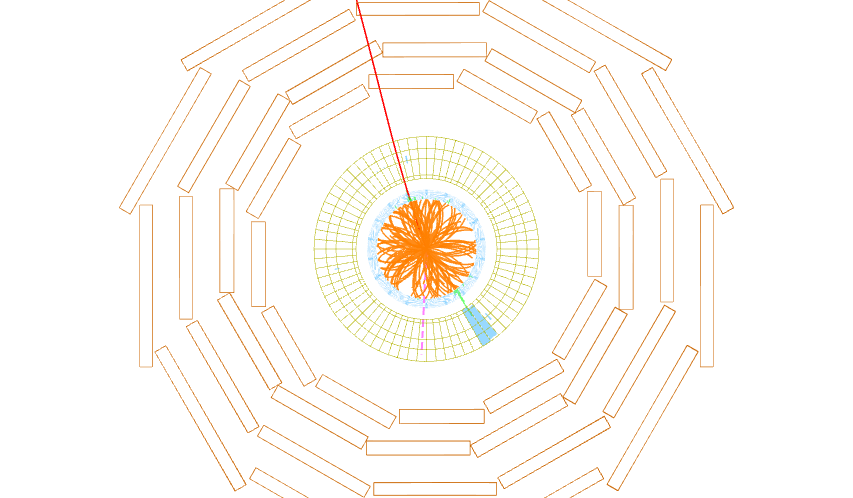
\includegraphics[width=\graphw,height=\graphh,keepaspectratio]{\PhDthesisdir/tex/slides/SM_MSSM_HTT_pheno/event_display/Event_1429090375_xy_white_struct_tracks.png}

\vfill

{\tiny
CMS record, Aug. 18, 2012, 14:37:39.352716 GMT
\qquad
Run 201191, Event 1429090375, LS 1071, xy plane.
}
\end{frame}


%\subsection*{Jet energy calibration}

\begin{frame}
\begin{minipage}[t]{.45\textwidth}
\begin{center}
\manip Niveaux de connaissance

\vspace{.5\baselineskip}

\begin{tabular}{rl}
particule & (\ptcl)\\
reconstruit & (\reco)\\
corrigé & (\cali)
\end{tabular}
\end{center}
\end{minipage}
\hfill\pause
\begin{minipage}[t]{.45\textwidth}
\begin{center}
\manip Réponse d'un jet
\begin{equation*}
R = \frac{\pT}{\pT_\ptcl}
\end{equation*}
\end{center}
\end{minipage}
\end{frame}


\begin{frame}[t]
%\transdissolve
\large
\includegraphics[width=\textwidth]{\PhDthesisdir/plots_and_images/from_JERC_RunI/CMS-JME-13-004_Figure_002-FR-TeX-sequential_for_slides/1.tex}

\vfill

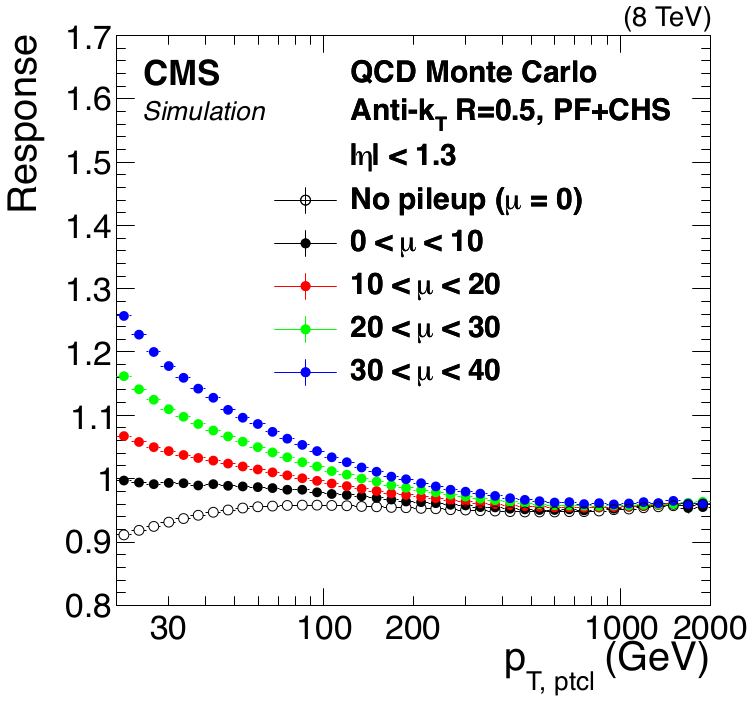
\includegraphics[height = \textheight/2]{\PhDthesisdir/plots_and_images/from_JERC_RunI/response_evolution_1.png}
\hfill
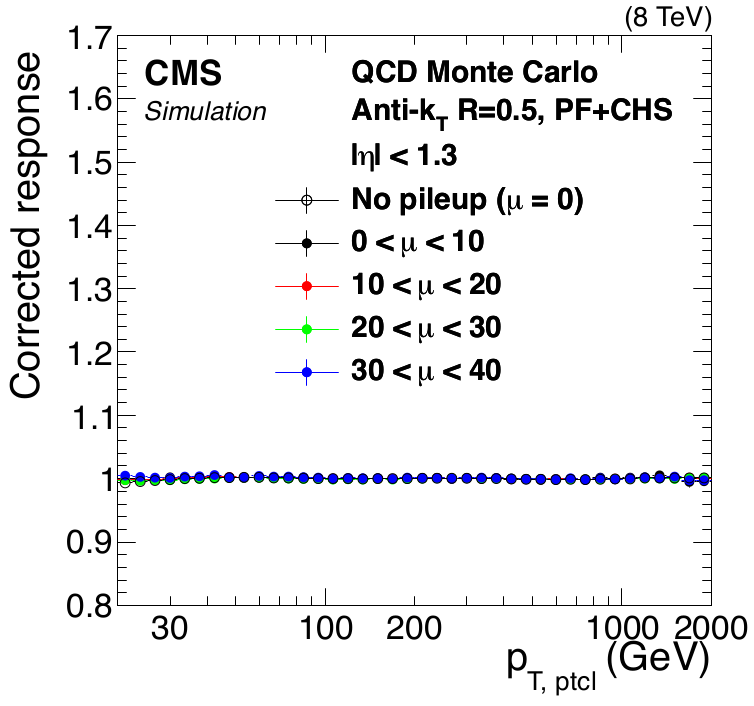
\includegraphics[height = \textheight/2]{\PhDthesisdir/plots_and_images/from_JERC_RunI/response_evolution_3.png}
\end{frame}

\begin{frame}[t]
\addtocounter{framenumber}{-1}
%\transdissolve
\large
\includegraphics[width=\textwidth]{\PhDthesisdir/plots_and_images/from_JERC_RunI/CMS-JME-13-004_Figure_002-FR-TeX-sequential_for_slides/2.tex}

\vfill

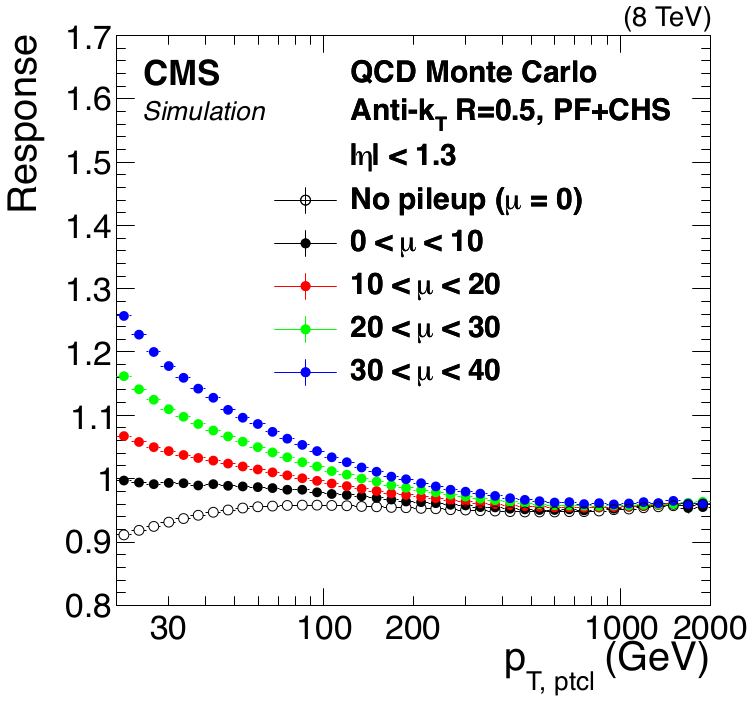
\includegraphics[height = \textheight/2]{\PhDthesisdir/plots_and_images/from_JERC_RunI/response_evolution_1.png}
\hfill
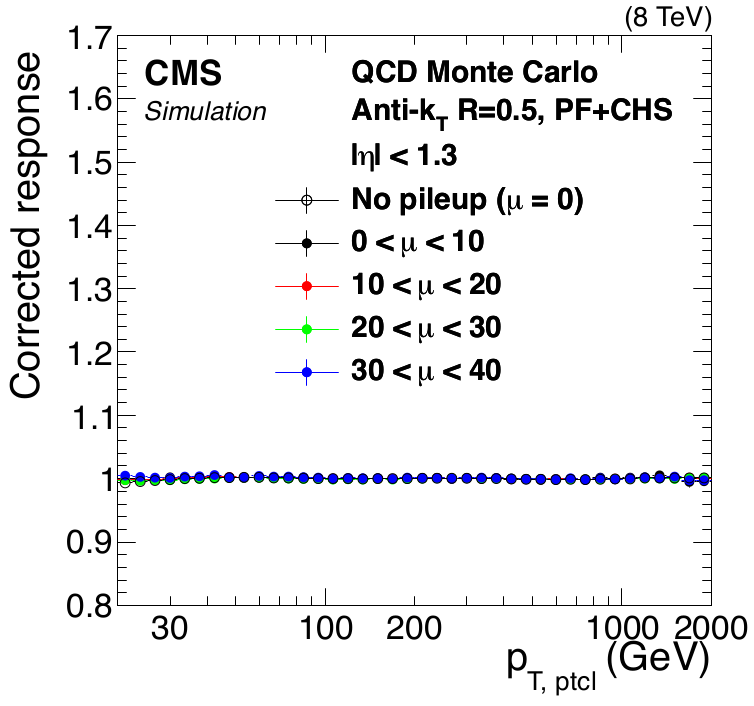
\includegraphics[height = \textheight/2]{\PhDthesisdir/plots_and_images/from_JERC_RunI/response_evolution_3.png}
\end{frame}

\begin{frame}[t]
\addtocounter{framenumber}{-1}
%\transdissolve
\large
\includegraphics[width=\textwidth]{\PhDthesisdir/plots_and_images/from_JERC_RunI/CMS-JME-13-004_Figure_002-FR-TeX-sequential_for_slides/3.tex}

\vfill

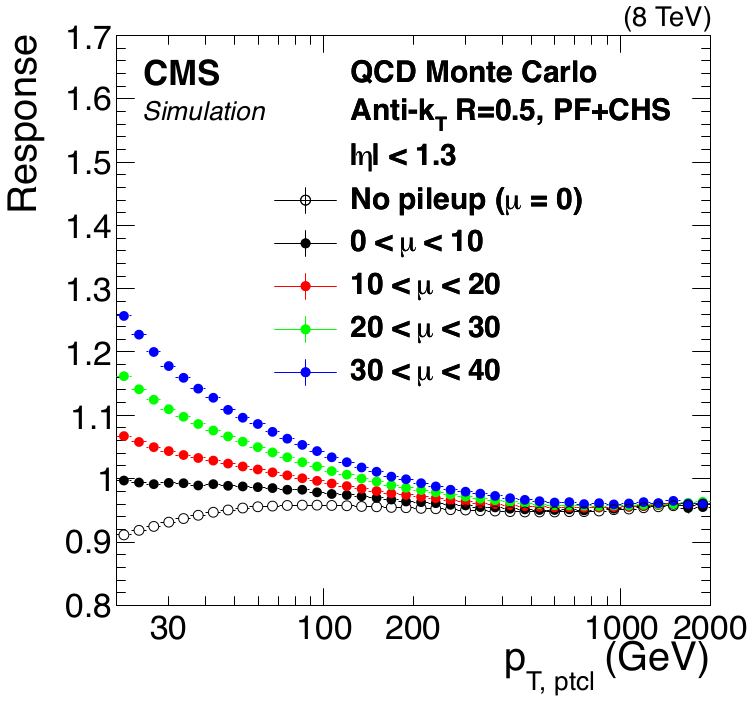
\includegraphics[height = \textheight/2]{\PhDthesisdir/plots_and_images/from_JERC_RunI/response_evolution_1.png}
\hfill
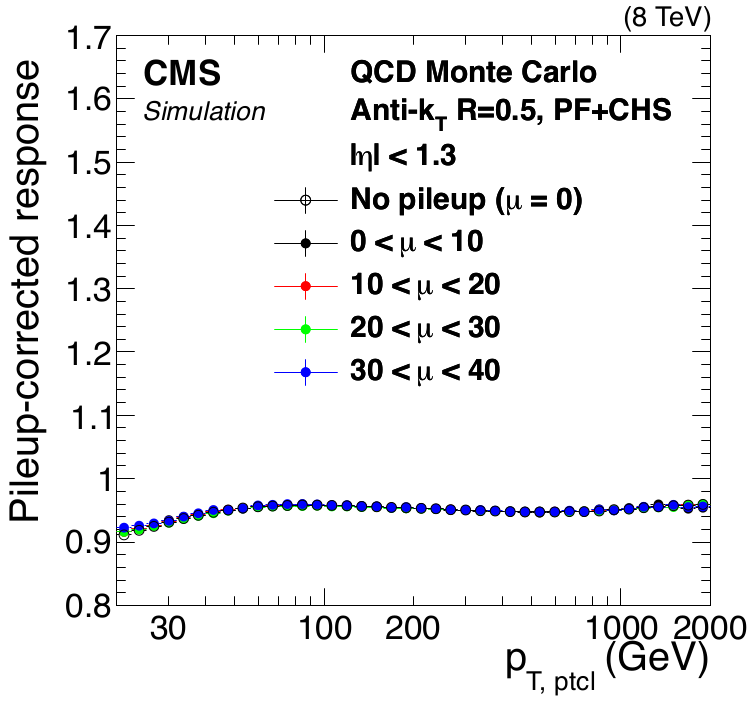
\includegraphics[height = \textheight/2]{\PhDthesisdir/plots_and_images/from_JERC_RunI/response_evolution_2.png}
\hfill
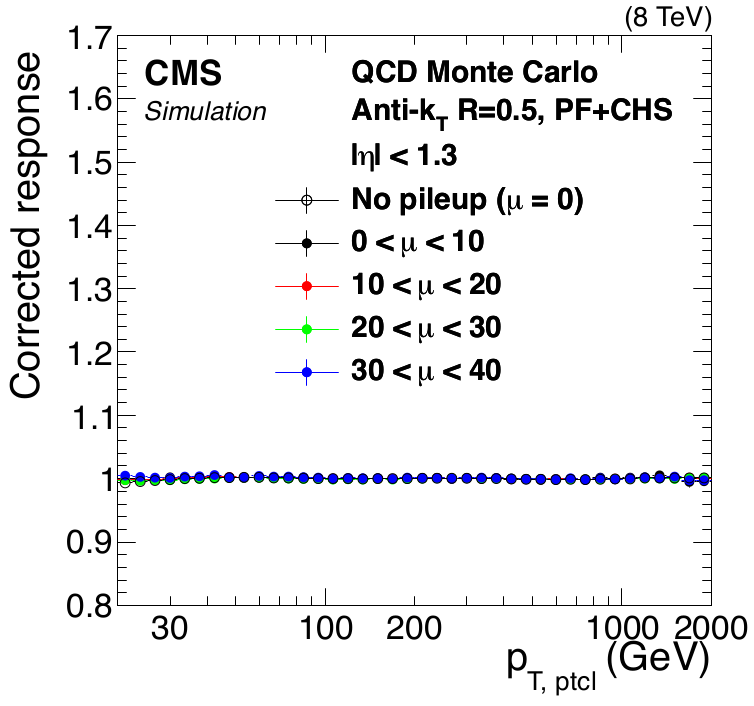
\includegraphics[height = \textheight/2]{\PhDthesisdir/plots_and_images/from_JERC_RunI/response_evolution_3.png}
\end{frame}

\begin{frame}[t]
\addtocounter{framenumber}{-1}
%\transdissolve
\large
\includegraphics[width=\textwidth]{\PhDthesisdir/plots_and_images/from_JERC_RunI/CMS-JME-13-004_Figure_002-FR-TeX-sequential_for_slides/4.tex}

\vfill

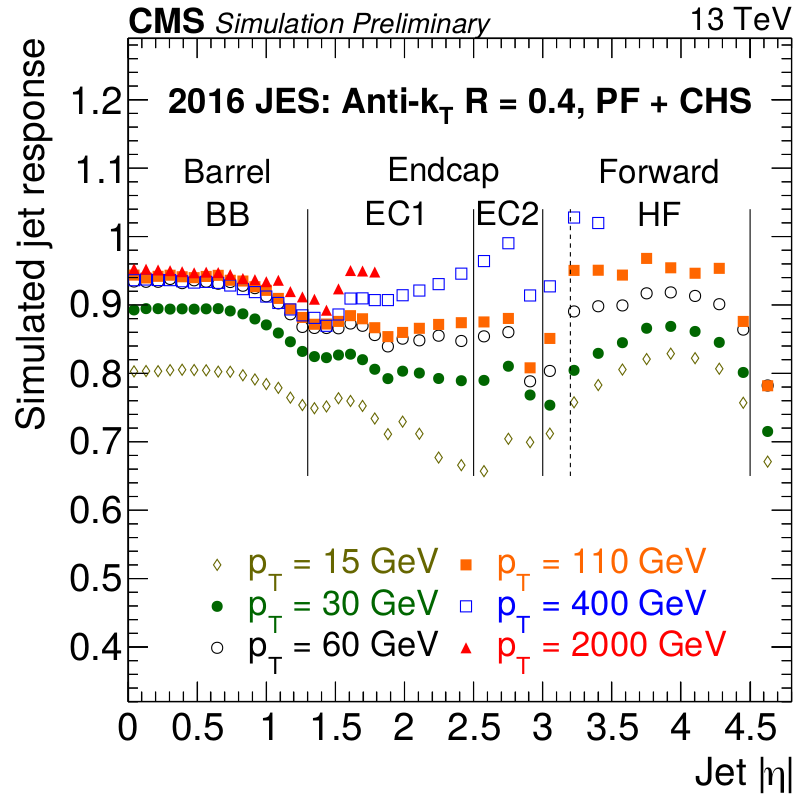
\includegraphics[height = \textheight/2]{\PhDthesisdir/plots_and_images/from_CMS-DP-2020-019/simulated_jet_response_2016.png}
\hfill
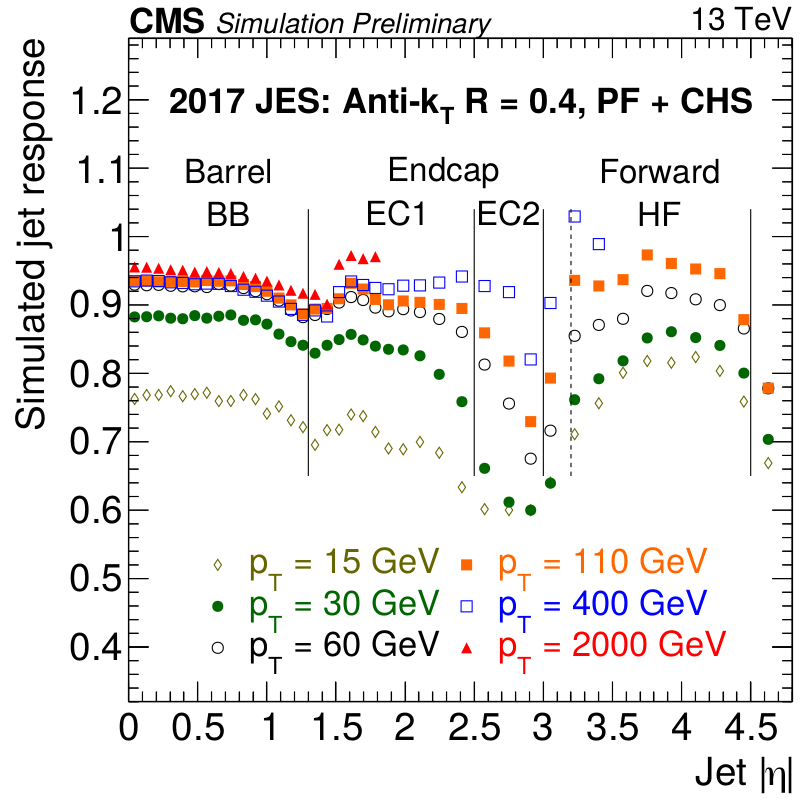
\includegraphics[height = \textheight/2]{\PhDthesisdir/plots_and_images/from_CMS-DP-2020-019/simulated_jet_response_2017.png}
\hfill
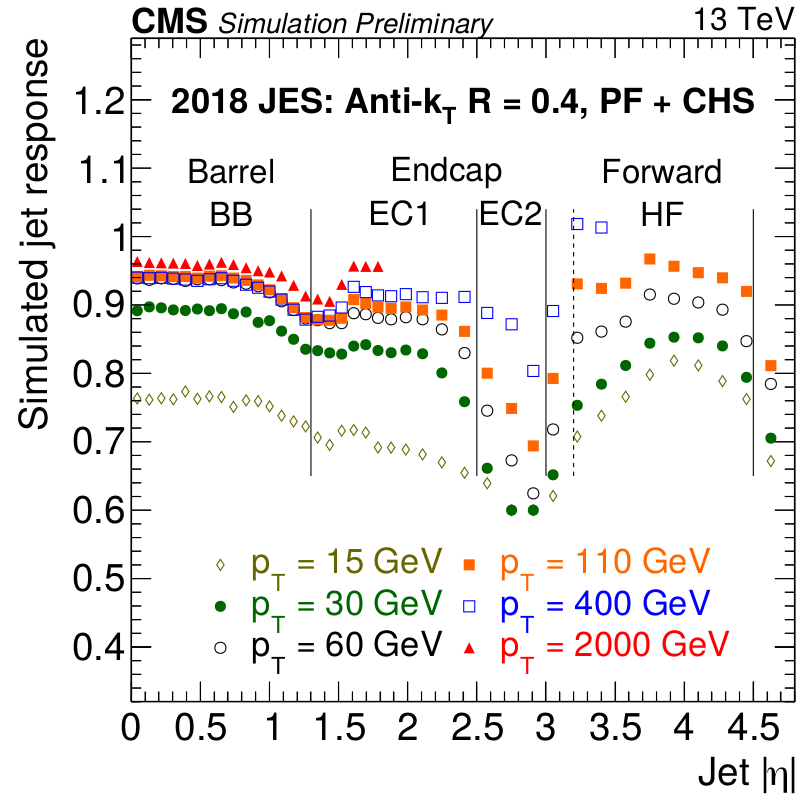
\includegraphics[height = \textheight/2]{\PhDthesisdir/plots_and_images/from_CMS-DP-2020-019/simulated_jet_response_2018.png}
\end{frame}

\begin{frame}[t]
\addtocounter{framenumber}{-1}
%\transdissolve
\large
\includegraphics[width=\textwidth]{\PhDthesisdir/plots_and_images/from_JERC_RunI/CMS-JME-13-004_Figure_002-FR-TeX-sequential_for_slides/5.tex}
\end{frame}

\begin{frame}[t]
\addtocounter{framenumber}{-1}
%\transdissolve
\large
\includegraphics[width=\textwidth]{\PhDthesisdir/plots_and_images/from_JERC_RunI/CMS-JME-13-004_Figure_002-FR-TeX-sequential_for_slides/6.tex}

\vfill

\includegraphics[height = \textheight/2]{\PhDthesisdir/plots_and_images/from_CMS-DP-2020-019/absolute_pT_residual_2016.png}
\hfill
\includegraphics[height = \textheight/2]{\PhDthesisdir/plots_and_images/from_CMS-DP-2020-019/absolute_pT_residual_2017.png}
\hfill
\includegraphics[height = \textheight/2]{\PhDthesisdir/plots_and_images/from_CMS-DP-2020-019/absolute_pT_residual_2018.png}
\end{frame}

\begin{frame}[t]
\addtocounter{framenumber}{-1}
%\transdissolve
\large
\includegraphics[width=\textwidth]{\PhDthesisdir/plots_and_images/from_JERC_RunI/CMS-JME-13-004_Figure_002-FR-TeX.tex}

\vfill

\begin{center}
\includegraphics[height = \textheight/2]{\PhDthesisdir/plots_and_images/from_JERC_RunI/Figure_030-a.png}
\end{center}
\end{frame}



%\input{\PhDthesisdir/slides/JERC/JEC_Principe/slides_anims/Gamma_plus_jet.tex}
\begin{frame}
\begin{center}
\includegraphics[width=\graphw,height=\graphh,keepaspectratio]{\PhDthesisdir/plots_and_images/Event_displays/JERC/Gamma_plus_jet.tex}
\end{center}
\end{frame}

\begin{frame}[t]
\vspace{\baselineskip}

~\hfill
\input{\PhDthesisdir/plots_and_images/Feynman_diagrams/Gamma_plus_jets/fgraph-gq_qGamma_S.tex}
\hfill\hfill\hfill
\input{\PhDthesisdir/plots_and_images/Feynman_diagrams/Gamma_plus_jets/fgraph-gq_qGamma_T.tex}
\hfill\hfill\hfill
\input{\PhDthesisdir/plots_and_images/Feynman_diagrams/Gamma_plus_jets/fgraph-qq_gGamma.tex}
\hfill~

\pause
\vfill

\begin{equation*}
\vpT_\ptcl^{\photon} + \vpT_\ptcl^\text{jet} = \vec{0}
\Rightarrow
\pT_\ptcl^{\photon} = \pT_\ptcl^\text{jet}
\end{equation*}
\pause
\begin{equation*}
R
= \frac{\pT_\reco^\text{jet}}{\pT_\ptcl^\text{jet}}
= \frac{\pT_\reco^\text{jet}}{\pT_\ptcl^{\photon}}
\simeq \frac{\pT_\reco^\text{jet}}{\pT_\reco^{\photon}}
\end{equation*}
\pause
\begin{equation*}
\Rbal = \frac{\pT_\reco^\text{jet}}{\pT^{\photon}}
\end{equation*}

%\manip Only 2 \og particles \fg{} (physics objects) in final state:
%\begin{itemize}
%\item photon (well known);
%\item jet (to calibrate).
%\end{itemize}
%\manip No neutrino $\Rightarrow$ no real \MET.
\end{frame}

%\input{\PhDthesisdir/slides/JERC/JEC_Principe/slides_anims/Gamma_plus_2jets.tex}
\begin{frame}
\begin{center}
\includegraphics[width=\graphw,height=\graphh,keepaspectratio]{\PhDthesisdir/plots_and_images/Event_displays/JERC/Gamma_plus_2jets.tex}
\end{center}
\end{frame}

\begin{frame}[t]
\vspace{\baselineskip}

~\hfill
\input{\PhDthesisdir/plots_and_images/Feynman_diagrams/Gamma_plus_jets/fgraph-gq_qGamma_T.tex}
\hfill~

\pause
\vfill

~\hfill
\input{\PhDthesisdir/plots_and_images/Feynman_diagrams/Gamma_plus_jets/fgraph-gq_qGamma_S-ISR_2jets.tex}
\hfill\hfill\hfill
\input{\PhDthesisdir/plots_and_images/Feynman_diagrams/Gamma_plus_jets/fgraph-gq_qGamma_S-ISR_2photons.tex}
\hfill\hfill\hfill
\input{\PhDthesisdir/plots_and_images/Feynman_diagrams/Gamma_plus_jets/fgraph-gq_qGamma_S-FSR_2jets.tex}
\hfill\hfill\hfill
\input{\PhDthesisdir/plots_and_images/Feynman_diagrams/Gamma_plus_jets/fgraph-gq_qGamma_S-FSR_2photons.tex}
\hfill~

\end{frame}

\begin{frame}
\begin{minipage}[t]{.45\textwidth}
\begin{equation*}
\Rbal = \frac{\pT_\reco^\text{jet 1}}{\pT^{\photon}}
\end{equation*}
\end{minipage}
\hfill
\begin{minipage}[t]{.45\textwidth}
\begin{equation*}
\alpha = \frac{\pT_\reco^\text{jet 2}}{\pT^{\photon}}
\end{equation*}
\end{minipage}
\end{frame}

\begin{frame}

\begin{equation*}
\vpT^\photon_\ptcl + \vpT^\text{recul}_\ptcl = \vec{0}
\end{equation*}

\pause
\vfill


\begin{equation*}
\vpT^\photon_\reco + \underbrace{\RMPF \vpT^\text{recul}_\ptcl}_{\vpT^\text{recul}_\reco} = -\vMET
\Rightarrow
\boxed{\RMPF = 1 + \frac{\vpT^\photon\cdot\vMET}{\abs{\vpT^\photon}^2}}
\end{equation*}
\end{frame}
\begin{frame}
\frametitle{$\photon+\text{jet}$ events: jet calibration, balancing method}
\manip The physics of the events gives
\begin{equation*}
\vpT^\photon_\ptcl + \vpT^\text{jet}_\ptcl = \vec{0} \Rightarrow \boxed{{\pT}^\photon_\ptcl = {\pT}^\text{jet}_\ptcl}
\end{equation*}

\pause
\vfill

\manip For the reconstructed objects, the balancing response is then defined as
\begin{equation*}
\vpT^\photon_\reco + \underbrace{\Rbal \vpT^\text{jet}_\ptcl}_{\vpT^\text{jet}_\reco} = \vec{0}
\Rightarrow
\boxed{\Rbal = \frac{{\pT}^\text{jet}_\reco}{\pT^\photon}}
\end{equation*}
\begin{equation*}
\text{because }
\pT^\photon_\ptcl\simeq\pT^\photon_\reco
=\pT^\photon
\mend
\end{equation*}
\end{frame}

\begin{frame}
\frametitle{$\photon+\text{jet}$ events: world is not perfect}
\begin{center}
\includegraphics[width=\graphw,height=\graphh,keepaspectratio, trim = 5.5cm 2cm 7.5cm 1.75cm, clip]{\PhDthesisdir/tex/slides/JERC/JEC_Principe/Gamma_plus_two_jets.pdf}
\end{center}
\end{frame}

\begin{frame}
\frametitle{$\photon+\text{jet}$ events: world is not perfect}
\manip Imbalance due to the presence of additionnal jets.
\pause
\manip Use the jet with higher \pT: $\displaystyle \boxed{\Rbal = \frac{{\pT}^\text{1\up{st}jet}_\reco}{\pT^\photon}}$.
\pause
\manip To avoid correction on additonnal jets: define $\displaystyle \boxed{\alpha = \frac{{\pT}^\text{2\up{nd}jet}_\reco}{\pT^\photon}}$ and extrapolate to $\alpha=0$.
\end{frame}

\begin{frame}
\frametitle{$\photon+\text{jet}$ events: jet calibration, MPF method}
\manip Considering balance between photon and \emph{all other particles},
\begin{equation*}
\vpT^\photon_\ptcl + \vpT^\text{recoil}_\ptcl = \vec{0}
\end{equation*}

\pause
\vfill

\manip For the reconstructed objects, the MPF response is then defined as
\begin{equation*}
\vpT^\photon_\reco + \underbrace{\RMPF \vpT^\text{recoil}_\ptcl}_{\vpT^\text{recoil}_\reco} = -\vMET
\Rightarrow
\boxed{\RMPF = 1 + \frac{\vpT^\photon\cdot\vMET}{\abs{\vpT^\photon}^2}}
\end{equation*}
\end{frame}
\begin{frame}
\frametitle{Run 2018 ABCD responses, $\alpha=\num{0.15}$, $\eta\in [\num{0},\num{1.3}]$}
\begin{minipage}{.45\textwidth}
\begin{figure}
\includegraphics[width=.9\linewidth]{\PhDthesisdir/contents/chapter-JERC/plots/2019-07-25/only_L2Res/Run2018ABCD/alpha_0_15/response_eta0013_balancing.pdf}
\caption{Balancing}
\end{figure}
\end{minipage}
\hfill
\begin{minipage}{.45\textwidth}
\begin{figure}
\includegraphics[width=.9\linewidth]{\PhDthesisdir/contents/chapter-JERC/plots/2019-07-25/only_L2Res/Run2018ABCD/alpha_0_15/response_eta0013_mpf.pdf}
\caption{MPF}
\end{figure}
\end{minipage}
\end{frame}

\begin{frame}
\frametitle{Run 2018 ABCD responses, extrapolation, $\pT\in [\num{175},\num{230}]\SI{}{\GeV}$, $\eta\in [\num{0},\num{1.3}]$}
\begin{minipage}{.45\textwidth}
\begin{figure}
\includegraphics[width=.9\linewidth]{\PhDthesisdir/contents/chapter-JERC/plots/2019-07-25/only_L2Res/Run2018ABCD/extrapolation/response_eta0013_ptPhot_175_230.pdf}
\caption{Balancing}
\end{figure}
\end{minipage}
\hfill
\begin{minipage}{.45\textwidth}
\begin{figure}
\includegraphics[width=.9\linewidth]{\PhDthesisdir/contents/chapter-JERC/plots/2019-07-25/only_L2Res/Run2018ABCD/extrapolation/responseMPF_eta0013_ptPhot_175_230.pdf}
\caption{MPF}
\end{figure}
\end{minipage}
\end{frame}

\begin{frame}
\frametitle{Run 2018 ABCD responses, extrapolated, $\eta\in [\num{0},\num{1.3}]$}
\begin{minipage}{.45\textwidth}
\begin{figure}
\includegraphics[width=.9\linewidth]{\PhDthesisdir/contents/chapter-JERC/plots/2019-07-25/only_L2Res/Run2018ABCD/extrapolated/response_eta0013_balancing_extrap.pdf}
\caption{Balancing}
\end{figure}
\end{minipage}
\hfill
\begin{minipage}{.45\textwidth}
\begin{figure}
\includegraphics[width=.9\linewidth]{\PhDthesisdir/contents/chapter-JERC/plots/2019-07-25/only_L2Res/Run2018ABCD/extrapolated/response_eta0013_mpf_extrap.pdf}
\caption{MPF}
\end{figure}
\end{minipage}
\end{frame}


\begin{frame}
\frametitle{Jet Energy Resolution}
\manip Remember \Rbal\ definition,
\begin{equation*}
\Rbal = \frac{{\pT}^\text{1\up{st}jet}_\text{reco}}{\pT^\photon_\text{reco}}
\end{equation*}

\pause

Then
\begin{equation*}
\Rbal
=
\underbrace{\frac{{\pT}^\text{1\up{st}jet}_\text{reco}}{{\pT}^\text{1\up{st}jet}_\text{ptcl}}}_{\sigma_\text{jet}=\text{JER}}
\times
\underbrace{\frac{{\pT}^\text{1\up{st}jet}_\text{ptcl}}{\pT^\photon_\text{ptcl}}
\vphantom{\frac{{\pT}^\text{1\up{st}jet}_\text{reco}}{{\pT}^\text{1\up{st}jet}_\text{ptcl}}}}_{\text{PLI}}
\times
\underbrace{\frac{\pT^\photon_\text{ptcl}}{\pT^\photon_\text{reco}}
\vphantom{\frac{{\pT}^\text{1\up{st}jet}_\text{reco}}{{\pT}^\text{1\up{st}jet}_\text{ptcl}}}}_{\sigma_\photon\equiv1}
\end{equation*}
\manip PLI: Particle Level Imbalance (pile-up, radiations, neutrinos...), $\to0$ when $\alpha\to0$.

\pause
\begin{equation*}
\boxed{\text{JER} = \sigma_\text{jet} =  \sqrt{\sigma_\Rbal^2 - \sigma_\text{PLI}^2}}
\end{equation*}
\end{frame}


\begin{frame}
\frametitle{Run 2018 ABCD jet resolution}
\begin{minipage}{.45\textwidth}
\begin{figure}
\includegraphics[width=\linewidth]{\PhDthesisdir/plots_and_images/my_plots/JERC/JER/Run2018ABCD/extrapolation/resolution_eta0005_ptPhot_400_500.pdf}
\caption{Extrapolation}
\end{figure}
\end{minipage}
\hfill
\begin{minipage}{.45\textwidth}
\begin{figure}
\includegraphics[width=\linewidth]{\PhDthesisdir/plots_and_images/my_plots/JERC/JER/Run2018ABCD/alpha_0_3/fine_eta_binning_Scale_factor_res_vs_ETA.pdf}
\caption{Scale factor}
\end{figure}
\end{minipage}
\end{frame}

\begin{frame}\addtocounter{framenumber}{-1}
\frametitle{Run 2018 ABCD jet resolution}
\begin{minipage}{.45\textwidth}
\begin{figure}
\includegraphics[width=\linewidth, trim=0cm 0cm 3cm 0cm]{\PhDthesisdir/plots_and_images/from_CMS_alignment_photodetectors/CMS-eta-ranges.png}
\caption{CMS and $\eta$ values}
\end{figure}
\end{minipage}
\hfill
\begin{minipage}{.45\textwidth}
\begin{figure}
\includegraphics[width=\linewidth]{\PhDthesisdir/plots_and_images/my_plots/JERC/JER/Run2018ABCD/alpha_0_3/fine_eta_binning_Scale_factor_res_vs_ETA.pdf}
\caption{Scale factor}
\end{figure}
\end{minipage}
\end{frame}



\subsection*{}
\section{$\Higgs\to\tau\tau$ analysis}
 


\subsection*{}
\section*{}
\begin{frame}

\begin{minipage}[t]{.45\textwidth}
\manip Remember: invariant mass not fully available:
\submanip neutrinos in di-\tau\ events.
\pause
\begin{block}{What's here}
\begin{center}
{\small (e.g. VBF Higgs production + decay to \tau\tau, \mu\tauh\ channel)}

\vspace{.5\baselineskip}

    \begin{tikzpicture}[scale=.8]
        \clip (-.5\linewidth,-.3\linewidth) rectangle (.5\linewidth,.3\linewidth);

        %\drawCMS

        %\printantimuondeposit{21}{15}
        \printantimuon{21}{15}
        
        \printneutrino[\antinutau]{30}
        \printneutrino[\numu]{-10}

        %\printjetdeposit{50}{170}
        \printjet{50}{170}

        %\printbigjetdeposit{150}{-50}
        \printbigjet{150}{-50}

        %\printtauhdeposit{15}{-150}
        \printtauh{15}{-150}
        
        \printneutrino[\nutau]{127}
    \end{tikzpicture}
\end{center}
\end{block}

\only<4->{
\manip It would be great to have a di-\tau\ mass estimator!
\submanip What about \emph{\textbf{machine learning}}?
}
\end{minipage}
\hfill
\begin{minipage}[t]{.45\textwidth}
\vspace{-\baselineskip}
\begin{block}{What CMS sees}
\begin{center}
\begin{center}
    \begin{tikzpicture}[scale=.45]
        \clip (0,0) circle (\muonroutd);

        \drawCMS

        \printantimuondeposit{21}{15}
        \printantimuontrk{21}{15}
%        \printantimuon{21}{15}

        \printjetdeposit{50}{170}
        \printjettrk{50}{170}
%        \printjetnolabel{50}{170}

        \printbigjetdeposit{150}{-50}
        \printbigjettrk{150}{-50}
%        \printbigjetnolabel{150}{-50}

        \printtauhdeposit{15}{-150}
        \printtauhtrk{15}{-150}
%        \printtauh{15}{-150}
        
        \draw [thick, ltcolorred, -latex] (0,0) --+ (75:.3\linewidth) node [right] {\vMET};
    \end{tikzpicture}
\end{center}
\end{center}
\end{block}
\end{minipage}

\begin{tikzpicture}[overlay, remember picture]
\only<-2>{
\fill [white] (.5\textwidth, -.1\textheight) rectangle (1.1\textwidth, .975\textheight);
}
\end{tikzpicture}
\end{frame}

\subsection*{}
\section{Machine learning}
\subsection{Event topology}
\begin{frame}%{Event topology (no PU considered)}

\begin{minipage}[c]{.275\textwidth}
\begin{block}{Higgs production}
\begin{center}
\small

\vspace{\baselineskip}

\begin{fmffile}{gg_loop_H_small_beamer}\fmfstraight
\begin{fmfchar*}(20,10)
  \fmfleft{g1,fi,g2}
  \fmfright{fo1,h,fo2}
  \fmf{gluon}{g1,g1loop}
  \fmf{gluon}{g2,g2loop}
  \fmf{phantom, tension=.6}{g1loop,fo1}
  \fmf{phantom, tension=.6}{g2loop,fo2}
  \fmffreeze
  \fmf{fermion}{g1loop,hloop,g2loop,g1loop}
  \fmf{fermion}{g2loop,g1loop}
  \fmf{dashes, tension=1.75}{hloop,h}
  \fmfdot{g1loop,hloop,g2loop}
  \fmffreeze
  \fmf{phantom}{g1loop,fakev1}
  \fmf{phantom}{g2loop,fakev1}
  \fmffreeze
%  \fmf{phantom,tension=1.5}{hloop,fakev2}
%  \fmf{phantom, label=$t,,\bar{t}$, l.side=left}{fakev1,fakev2}
%  \fmf{phantom, label=$b,,\bar{b}$, l.side=right}{fakev1,fakev2}
  \fmflabel{\gluon}{g1}
  \fmflabel{\gluon}{g2}
  \fmflabel{\Hn}{h}
\end{fmfchar*}
\end{fmffile}


\vspace{2\baselineskip}

\begin{fmffile}{bg_b_bH_small_beamer}\fmfstraight
\begin{fmfchar*}(20,10)
  \fmfleft{i1,i2}
  \fmfright{o1,o2}
  \fmf{fermion}{i2,v1,v2,o1}
  \fmf{gluon}{i1,v1}
  \fmf{dashes}{v2,o2}
  \fmfdot{v1,v2}
  \fmflabel{\gluon}{i1}
  \fmflabel{\quarkb}{i2}
  \fmflabel{\quarkb}{o1}
  \fmflabel{\Hn}{o2}
\end{fmfchar*}
\end{fmffile}

\vspace{2\baselineskip}

\begin{fmffile}{gg_Hbb_small_beamer}\fmfstraight
\begin{fmfchar*}(20,10)
  \fmfleft{g1,g2}
  \fmfright{b1,h,b2}
  \fmf{gluon}{g1,g1b1}
  \fmf{gluon}{g2,g2b2}
  \fmf{fermion}{g1b1,b1}
  \fmf{fermion}{b2,g2b2}
  \fmffreeze
  \fmf{fermion}{g2b2,bh,g1b1}
  \fmffreeze
  \fmf{dashes}{bh,h}
  \fmfdot{g1b1,g2b2,bh}
  \fmflabel{\gluon}{g1}
  \fmflabel{\gluon}{g2}
  \fmflabel{\quarkb}{b1}
  \fmflabel{\antiquarkb}{b2}
  \fmflabel{\Hn}{h}
\end{fmfchar*}
\end{fmffile}


\vspace{\baselineskip}

...
\end{center}
\end{block}
\end{minipage}
\hfill%\pause
\begin{minipage}[c]{.04\textwidth}
\begin{center}
\large$\times$
\end{center}
\end{minipage}
\hfill
\begin{minipage}[c]{.275\textwidth}
\begin{block}{$\Higgs\to\tau\tau$}
\begin{center}
\vspace{\baselineskip}
\begin{fmffile}{H-tautau_small_beamer}\fmfstraight
\begin{fmfchar*}(20,10)
  \fmfleft{h}
  \fmfright{tau1,tau2}
  \fmf{dashes}{h,v}
  \fmf{fermion}{tau1,v}
  \fmf{fermion}{v,tau2}
  \fmfdot{v}
  \fmflabel{\antitau}{tau1}
  \fmflabel{\leptau}{tau2}
  \fmflabel{\Hn}{h}
\end{fmfchar*}
\end{fmffile}
\vspace{\baselineskip}
\end{center}
\end{block}
\end{minipage}
\hfill%\pause
\begin{minipage}[c]{.04\textwidth}
\begin{center}
\large$\times$
\end{center}
\end{minipage}
\hfill
\begin{minipage}[c]{.275\textwidth}
\begin{block}{\tau\ decays}
\begin{center}

\vspace{\baselineskip}

\begin{fmffile}{tau_to_ele_small_beamer}%\fmfstraight
\begin{fmfchar*}(20,10)
  \fmfleft{taui}
  \fmfright{l1,l2,l3,f1,f2,f3,nuout}
  \fmf{fermion, tension=2}{taui,v1}
  \fmf{fermion}{v1,nuout}
  \fmf{phantom}{v1,l1}
  \fmffreeze
  \fmflabel{$\nutau$}{nuout}
  \fmf{boson, label=$\Wbosonminus$, l.side=right, tension=2}{v1,v2}
  \fmf{phantom}{v2,td1,l1}
  \fmf{phantom}{v2,td2,l2}
  \fmf{phantom}{v2,td3,l3}
  \fmffreeze
  \fmf{fermion}{l1,v2,l3}
  \fmflabel{\antinuele}{l1}
  \fmflabel{\electron}{l3}
  \fmflabel{\leptau}{taui}
  \fmfdot{v1,v2}
\end{fmfchar*}
\end{fmffile}


\vspace{2\baselineskip}

\begin{fmffile}{tau_to_mu}%\fmfstraight
\begin{fmfchar*}(30,20)
  \fmfleft{taui}
  \fmfright{l1,l2,nuout}
  \fmf{fermion, tension=2}{taui,v1}
  \fmf{fermion}{v1,nuout}
  \fmf{phantom}{v1,l1}
  \fmffreeze
  \fmflabel{$\nutau$}{nuout}
  \fmf{boson, label=$\Wbosonminus$, l.side=right, tension=2}{v1,v2}
  \fmf{fermion}{l2,v2,l1}
  \fmflabel{$\muon$}{l1}
  \fmflabel{$\antinumu$}{l2}
  \fmflabel{\leptau}{taui}
  \fmfdot{v1,v2}
\end{fmfchar*}
\end{fmffile}


\vspace{2\baselineskip}

\begin{fmffile}{tau_to_tauh_small_beamer}%\fmfstraight
\begin{fmfchar*}(20,10)
  \fmfleft{taui}
  \fmfright{l1,l2,l3,f1,f2,f3,nuout}
  \fmf{fermion, tension=2}{taui,v1}
  \fmf{fermion}{v1,nuout}
  \fmf{phantom}{v1,l1}
  \fmffreeze
  \fmflabel{$\nutau$}{nuout}
  \fmf{boson, label=$\Wbosonminus$, l.side=right, tension=2}{v1,v2}
  \fmf{phantom}{v2,td1,l1}
  \fmf{phantom}{v2,td2,l2}
  \fmf{phantom}{v2,td3,l3}
  \fmffreeze
  \fmf{plain}{td3,v2,td1}
  \fmfblob{.15w}{td2}
  \fmf{plain}{td2,l2}
  \fmflabel{\tauhm}{l2}
  \fmflabel{\leptau}{taui}
  \fmfdot{v1,v2}
\end{fmfchar*}
\end{fmffile}


\vspace{\baselineskip}

\end{center}
\end{block}
\end{minipage}

%\pause
\vfill

\begin{minipage}[c]{.275\textwidth}
\begin{center}
eventual jets
\end{center}
\end{minipage}
\hfill
\begin{minipage}[c]{.04\textwidth}

\end{minipage}
\hfill
\begin{minipage}[c]{.275\textwidth}
\begin{center}
\num{2} taus
\end{center}
\end{minipage}
\hfill
\begin{minipage}[c]{.04\textwidth}

\end{minipage}
\hfill
\begin{minipage}[c]{.275\textwidth}
\begin{center}
$\set{1,2}$ neutrinos per tau\\
$+ \set{\ele, \mu, \tauh}$
\end{center}
\end{minipage}

\end{frame}


\subsection*{ML models inputs}
\begin{frame}%{Stored observables}

\manip ML models inputs are based on reconstructed variables (what is available in real data).

\pause
\manip $\Higgs\to\tau\tau$ decays:
\submanip visible decay products $\to$ $\pT^{(1,2)}$, $\eta^{(1,2)}$ and $\phi^{(1,2)}$,
\submanip MET to account for neutrinos $\to$ \MET, $\phi^\text{MET}$;

\pause
\manip Higgs production:
\submanip two leading jets $\to$ $\pT^{(j1,j2)}$, $\eta^{(j1,j2)}$ and $\phi^{(j1,j2)}$;

\pause
\manip Higher level variables:
\submanip transverse masses $\mT^1$, $\mT^2$, $\mT^{\tau\tau}$,
\submanip total transverse mass \mTtot.

\pause
\manip Additionnal variables:
\submanip MET covariance matrix;
\submanip remaining jets overall $\vec{p}$ $\to$ $\pT^r$, $\eta^r$ and $\phi^r$;
\submanip number of neutrinos ($\tauh\tauh = 2$, $\ell\tauh=3$, $\ell\ell=4$);
\submanip number of PU vertices \inlinecode{python}{npvsGood};

%\vfill
%
%\pause
%\manip \todo{update above list with best model's inputs and compute numb. of} inputs.

\end{frame}


\subsection{NN structure}
\newcommand{\drawN}[2][c]{
\node [draw, circle] (#1) at (#2) {};
}

\def\linkN#1#2{
\draw [-latex] (#1) -- (#2);
}
\begin{frame}{(Deep) Neural Networks}
\begin{center}
\begin{tikzpicture}

\foreach \y in {0,1,2,-2}{
\foreach \x in {1,2,...,5}{
\drawN[\x\y]{\x,\y}
}
}

\foreach \yi/\N in {1.5/1,0.5/2,-1.5/n}{
\fill (-.5,\yi) circle(2pt) node [left] {$x_{\N}$};
\foreach \y in {0,1,2,-2}{
\draw [-latex] (-.5,\yi) -- (1\y);
}
}

\drawN[No]{6.5,0}

\draw [-latex] (No) --+ (.5,0) node [right] {$y=F(\vec{x})$};

\foreach \ya in {0,1,2,-2}{
\foreach \yb in {0,1,2,-2}{
\linkN{5\ya}{No}
\foreach \xa/\xb in {1/2,2/3,3/4,4/5}{
\linkN{\xa\ya}{\xb\yb}
}
}
}

\fill[white] (2.33,-2.5) rectangle (4.66,2.5);

\foreach \x/\y in {-.5/-.5,1/-1,2/-1,5/-1}{
\fill (\x,\y) circle (1pt);
\fill (\x,\y+.2) circle (1pt);
\fill (\x,\y-.2) circle (1pt);
}

\foreach \y in {0,1,2,-2}{
\fill (3.5,\y) circle (1pt);
\fill (3.5+.2,\y) circle (1pt);
\fill (3.5-.2,\y) circle (1pt);
}

\foreach \x in {.25,5.75}{
\draw [thick, dotted, CERNblue] (\x,-2.5) -- (\x,2.5);
}

\draw [CERNblue] (-.65, 2.5) node {Input layer\vphantom{Àq}};
\draw [CERNblue] (3, 2.5) node {Hidden layers\vphantom{Àq}};
\draw [CERNblue] (7.5, 2.5) node {Output layer\vphantom{Àq}};

\draw [thick, ltcolorred, latex-latex] (.25,-2.25) -- (5.75,-2.25);
\draw [ltcolorred] (3, -2.5) node {\NLayers\vphantom{Àq}};

\draw [thick, ltcolorred, latex-latex] (4.5,-2.125) -- (4.5,2.125);
\draw [ltcolorred] (4.5, 0) node [left] {\NNeurons\vphantom{Àq}};

\end{tikzpicture}

%\manip For us, $\NLayers =3$ and $\NNeurons =1000$.
\end{center}
\end{frame}

\subsection{NN training}
\begin{frame}
\manip \GeV\ switched to \TeV

\manip Target is $m_{\Higgs}$

\manip Get a flat target distribution for the training, validating and testing sub-samples.

\manip Train a NN for:
\submanip all channels at once;
\submanip each channel separately;
\submanip \todo{full-hadronic, semi-leptonic, full-leptonic} channels (categorize per amount of neutrinos in the final state).
\end{frame}

\subsection*{}
\section*{Conclusion \& prospects}
\begin{frame}{Conclusion \& prospects: \HAtoTauTau}
\manip MSSM \HAtoTauTau\ analysis on full Run~II:
\submanip 4 final states: \tauh\tauh, \mu\tauh, \ele\tauh\ and \ele\mu,
\submanip Model independent exclusion limits on $\sigma\times\BR$,
\submanip Model dependent exclusion contours in the $(m_{\HiggsA}, \tan\beta)$ plane.
\manip CMS paper HIG-21-001 on its way for publication:
\submanip Leading-edge until Run~III corresponding results!
\manip No evidence for MSSM.
\end{frame}

\begin{frame}{Conclusion \& prospects: ML project}
\manip Successful $m_{\higgsML}$ reconstruction in di-\tau\ events.
\submanip Not only MSSM \HAtoTauTau\ but any $X\to\tau\tau$ analysis could benefit from this project.
\manip \mml\ vs \mTtot:
\submanip A good mass estimator is not always a good discriminating variable.
\submanip Still, we already have the same performances at this point.
\manip \mml\ vs \msv:
\submanip Similar Higgs sensitivity for some event topologies.
\submanip Better \Zboson\ estimation observed (the model has been trained on $\higgsML\to\tau\tau$ with various masses only).
\submanip Could be improved by updating the training datasets (other kinds of events).
\submanip Faster (about 60 times!).
\manip Very promising as a di-\tau\ mass predictor (\SVFIT\ successor?).
\end{frame}

\newcounter{txtlines}
\newcommand{\drawCARD}[5][1]{ % defined coordinate, logo, width, txts
\draw (#2)+(-.5, .05) coordinate (tmp);
\setcounter{txtlines}{0}
\foreach \txt in {#5}{\stepcounter{txtlines}}
\fill [white, blur shadow={shadow blur steps=5}, rounded corners = 5pt] (#2) rectangle  +(#4, - 8 -\baselineskip*\thetxtlines);
\fill [white, blur shadow={shadow blur steps=5}, rounded corners = 3pt] (#2)+(#1/2+#4-#1/4, #1/2-#1/4) rectangle  +(- #1/2 +#4-#1/4, - #1/2-#1/4);
\begin{scope}
\clip [rounded corners = 3pt] (#2)+(#1/2+#4-#1/4, #1/2-#1/4) rectangle  +(- #1/2 +#4-#1/4, - #1/2-#1/4);
\ifthenelse{\equal{#3}{CMS_logo.pdf}}{
\draw (#2)+(#4 -#1/4, -#1/4) node {\includegraphics[height= #1 cm, width= #1 cm, keepaspectratio, trim = 2mm 2mm 2mm 2mm, clip]{\PhDthesisdir/plots_and_images/logos/#3}} ;
}{
\draw (#2)+(#4 -#1/4, -#1/4) node {\includegraphics[height= #1 cm, width= #1 cm, keepaspectratio]{\PhDthesisdir/plots_and_images/logos/#3}} ;
}
\end{scope}
\foreach \txt in {#5}{
\draw (tmp.west) + (0,-\baselineskip) node [right, text depth=0pt] (tmp) {\submanip \txt \vphantom{Àq}};
}

\draw (#2) + (0,- 8 -\baselineskip*\thetxtlines -15) coordinate (bottom);
\draw (#2) + (#4+.5,0) coordinate (right);
}
\begin{frame}{\emph{Merci !}}\thispagestyle{empty}
%\only<2->{\transdissolve}
%\only<-9>{\transduration{0}}
\begin{center}
\begin{tikzpicture}[overlay]

\draw (-1,4.25) coordinate (IP2I);
\drawCARD{IP2I}{logo_IP2I.pdf}{4}{Colin,{Gaël, Ece},Hugues,{Aurélien, Antoine L.},{Jean-François, Grégoire},{Corentin, Martin},autres doctorants,groupe CMS,Antoine C.,personnels}

\draw (bottom) coordinate (CMS);

\draw (right) coordinate (KIT);
\drawCARD{KIT}{KIT.png}{4}{{Günter, Roger},Artur,{Sebastian B., Maximilian}, Sebastian W., Janek, Felix}

\draw (bottom) coordinate (IC);
\drawCARD{IC}{IC.jpg}{4}{Daniel,David,George}

\draw (bottom) coordinate (DESY);
\drawCARD{DESY}{DESY.png}{4}{Aleksei,Mareike}

\draw (bottom) coordinate (HEPHY);
\drawCARD{HEPHY}{HEPHY-crop.png}{4}{Janik,Suman}

\drawCARD{CMS}{CMS_logo.pdf}{4}{équipe des guides,Jacob,Jean,Giuseppe,Juska,Yi,Mikko}

\draw (-4.5,2.25) node (MESRI) {\includegraphics[height=1.2 cm, keepaspectratio]{\PhDthesisdir/plots_and_images/logos/ES-R-I_horizontal.pdf}} ;

\draw (MESRI.south) + (0,-.75) node [below left] (PHAST) {\includegraphics[height=1.2 cm, keepaspectratio]{\PhDthesisdir/plots_and_images/logos/phast-logo.png}} ;

\draw (MESRI.south) + (0,-.75) node [below right] (UCBL) {\includegraphics[height=1.2 cm, keepaspectratio]{\PhDthesisdir/plots_and_images/logos/Planche_UdL_LogoLyon1Sig_CoulCmjnVecto-eps-converted-to.pdf}} ;

\draw (PHAST.south) + (0,-.75) node [below] (CNRS) {\includegraphics[height=1.2 cm, keepaspectratio]{\PhDthesisdir/plots_and_images/logos/IN2P3-B_SignV_bleu-eps-converted-to.pdf}} ;

\draw (UCBL.south) + (0,-.75) node [below] (CERN) {\includegraphics[height=1.2 cm, keepaspectratio]{\PhDthesisdir/plots_and_images/logos/CERN-logo.jpg}} ;

\end{tikzpicture}
\end{center}
\end{frame}